\chapter{Ontology implementation}
I this phase there is the actual implementation of prompt engineering ontology, starting from functional and non-functional requirements defined in the previous phase. The LOT methodology includes four steps: 
\begin{enumerate}
    \item Ontology conceptualization

    \item Ontology reuse

    \item Ontology encoding

    \item Ontology evaluation
\end{enumerate}
as we can see in the figure below:
\begin{figure}[H]
    \centering
    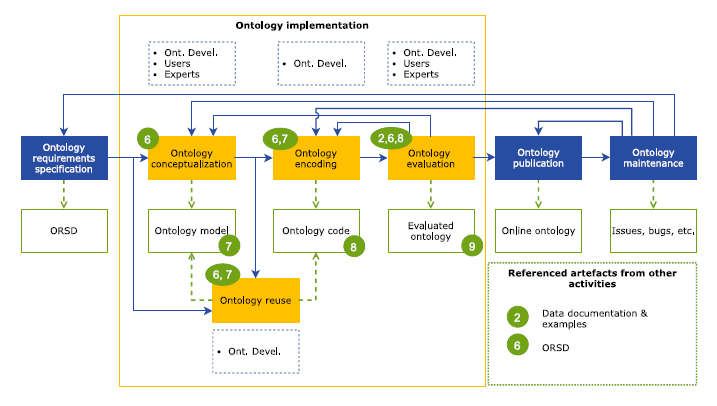
\includegraphics[width=0.9\linewidth]{Figures/fig_14.png}
    \caption{Ontology implementation workflow}
    \label{fig:enter-label}
\end{figure}
At the end of this phase, the output is an ontology read y to be published and to be made available online.

\newpage
\section{Ontology conceptualization}
The first step in the ontology implementation is the ontology conceptualization. In this phase there is the definition of all main concepts in the ontology with the relations among them. I used \href{draw.io}{https://app.diagrams.net/} software : a free easy-to-use diagramming tool that allows to represent UML diagrams and many more. I chose this software over other diagramming tools because it is intuitive, easy to use, and frequently updated moreover with draw.io it is possible to export diagrams in other formats like: svg, pdf and png in high resolution.\\
Starting from competency questions I chosed a top-down strategy in order to model the domain of prompt engineering and large language models, modeling first major concepts and then going more into detail. The idea behind the conceptualization of large language models is  taking the user's perspective: what informations are useful and meaningful to a user about large language models? From this perspective, I decided not to dwell too much on theoretical details but to focus on concepts that are useful for users in selecting the most suitable large language model for their purposes. A large language model is represented using four dimensions:
\begin{enumerate}
    \item \textbf{Type:} type of large language model which is a sub concept. Each type of large language model has one or more instances representing versions of that large language model.

    \item \textbf{Organization:} organization that creates the large language model.

    \item \textbf{Base model:} the deep learning model at the base of the architecture of the large language model. This concept represents a characteristic of a large language model.

    \item \textbf{Capability:} the capability of a large language model and it represents a characteristic of a large language model.
\end{enumerate}
These concepts provide a representation of various aspects of large language models, from their underlying architecture to the organizations that develop them, which can range from universities and research institutions to companies with business-oriented goals. A fundamental aspect is the representation of the capabilities of large language models. In fact, the ontology will not only include large language models capable of processing text but also multimodal models capable of handling more complex data types, such as images, audio, video, and source code.\\
Regarding prompt engineering, starting from the user's perspective, I decided to model the domain using the following concepts:
\begin{itemize}
    \item \textbf{Prompting technique:} this concept gathers all the prompting techniques, each prompting technique is a sub concept.

    \item \textbf{Prompt:} this is the base concept, a single prompt provided as input in the context of a chat with a specific large language model, followed by a response. The prompt can be generated using a prompting technique.

    \item \textbf{Chat:} this concept represents the context of a prompt with a specific large language model and it can include one or more prompts and responses.

    \item \textbf{Response:} this concepts reprents the response 
    generated by large language model after the input of a prompt in the context of a specific chat.
\end{itemize}
In addition there is also the modelling of the concept \textbf{"Task"} represents the tasks to be solved using large language models by applying prompting techniques. This concept has sub concepts specific for the task that has to be solved like: image task, text task, code task, audio task and video tasks, each one of those concepts has other sub concepts, for example the "text task" has as sub concepts: text summarization, emotion classification, text translation ecc. The concepts of \textbf{"Chat"} and \textbf{"Prompt"} are introduced to decouple each prompting technique from a specific large language model, ensuring their independence. The reasoning behind this conceptualization is simple and straightforward: a prompt is created using a specific prompting technique and applied in the context of a specific chat with a version of large language model producing a response. The connection with the concept of Task lies in solving a specific task through the use of an instance of a prompting technique.\\
Once defined the major concepts in the ontology, I define the relations between these concepts. Starting from the large language model, each sub concept like GPT, Mistral, Gemini is involved in the following relations:
\begin{itemize}
    \item \textit{develops:} an organization develops a large language model type, for example Google develops Gemini.

    \item \textit{has architecture:} a large language model type has architecture a specific base model, for example GPT has architecture the decoder-only model.

    \item \textit{has capability:} a large language model type has capability a specific capability and all versions have that capability. For example if GPT has capability the text processing capability, GPT-1, GPT-2, GPT-3 and GPT-4 are able to process text. In the case where a version represents an evolution of the model by introducing new capabilities, that specific version will be linked to the newly introduced capabilities, for example GPT-4 has \textit{image processing} and \textit{code processing} capabilities.
\end{itemize}
As we have seen, the aspect of different versions of the same model (GPT) must be considered and appropriately represented. To achieve this, I have used two distinct relations:
\begin{itemize}
    \item \textit{has variant:} this relation represents a contemporaneity between two models, where a model x is a variant of a model y, and this does not represent an evolution of model x. For example Mistral-7B has variant Codestral (a version of Mistral specific for source code processing.)

    \item \textit{evolves:} unlike \textit{has variant}, this relation represents a temporal succession between an older model and a newer model, for example GPT-3 evolves GPT-4, where GPT-4 is a more recent and powerful version of GPT. For this relation, I have introduced also the inverse relation \textit{evolved from}.
\end{itemize}
Another specific aspect considered is the presence of relations between organizations developing large language models, where one organization is part of another organization, for example, DeepMind is a research organization and is part of Google. I created two relations called: \textit{has organization} and \textit{is organization of} in order to represent this aspect in the ontology. In the figure below we can see the conceptualization of the part just described.
\begin{figure}[H]
    \centering
    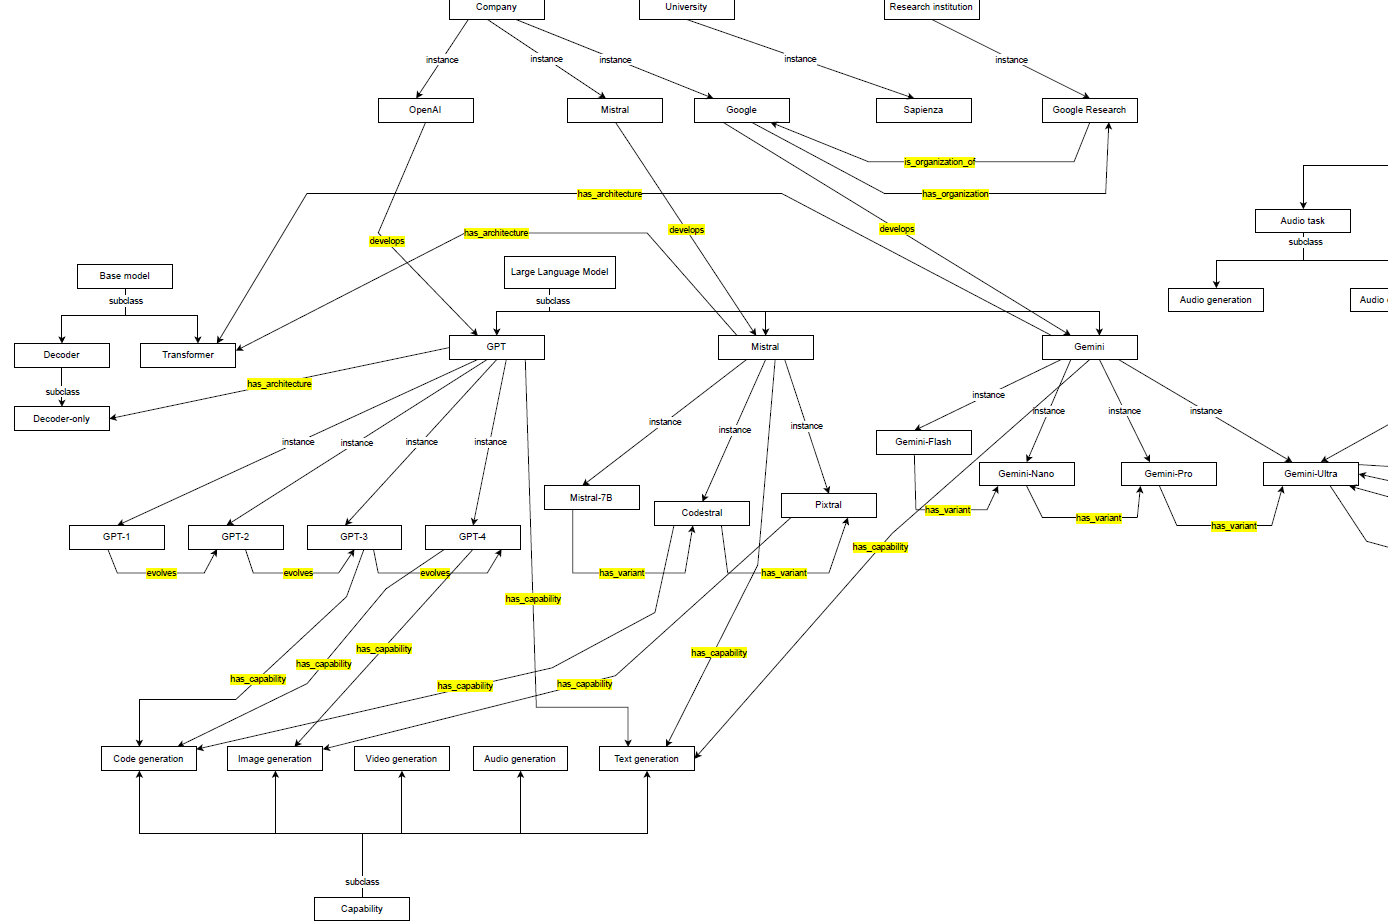
\includegraphics[width=0.9\linewidth]{Figures/fig_26.png}
    \caption{Large language models\\ dimensions conceptualization}
    \label{fig:enter-label}
\end{figure}
Regarding the prompt domain the following relations have been created in order to properly connect concepts introduced:
\begin{itemize}
    \item \textit{solves task:} this relation connects an instance of a prompting technique with an instance of a task, where the instance of the prompting technique solves that specific task. The inverse relation is: \textit{solved by}.

    \item \textit{is used in prompt:} the instance of a prompting technique is used in a specific prompt for generating the prompt using that technique. The inverse relation is: \textit{prompt generated using}.

    \item \textit{has context:} this relation connects the prompt with its context, the chat where one or more prompt are connected to. The inverse relation is: \textit{has prompt}.

    \item \textit{uses model:} this relation connects the chat with the specific model that is used to input prompts and generate responses. The inverse relation is: \textit{is used in chat}

    \item \textit{generates response:} this relation connects the specific large language model with the response generated after the input of the prompt. The inverse relation is: \textit{response generated using}.

    \item \textit{prompt follows response:} this relation connects a prompt with its response, the inverse relation is: \textit{response followed by prompt}.

    \item \textit{has response:} this relation connects the chat with the response generated by the model, the inverse relation is: \textit{is response of}. 
\end{itemize}
The conceptualization of prompt engineering domain is represented in the below diagram using draw.io

\begin{figure}[H]
    \centering
    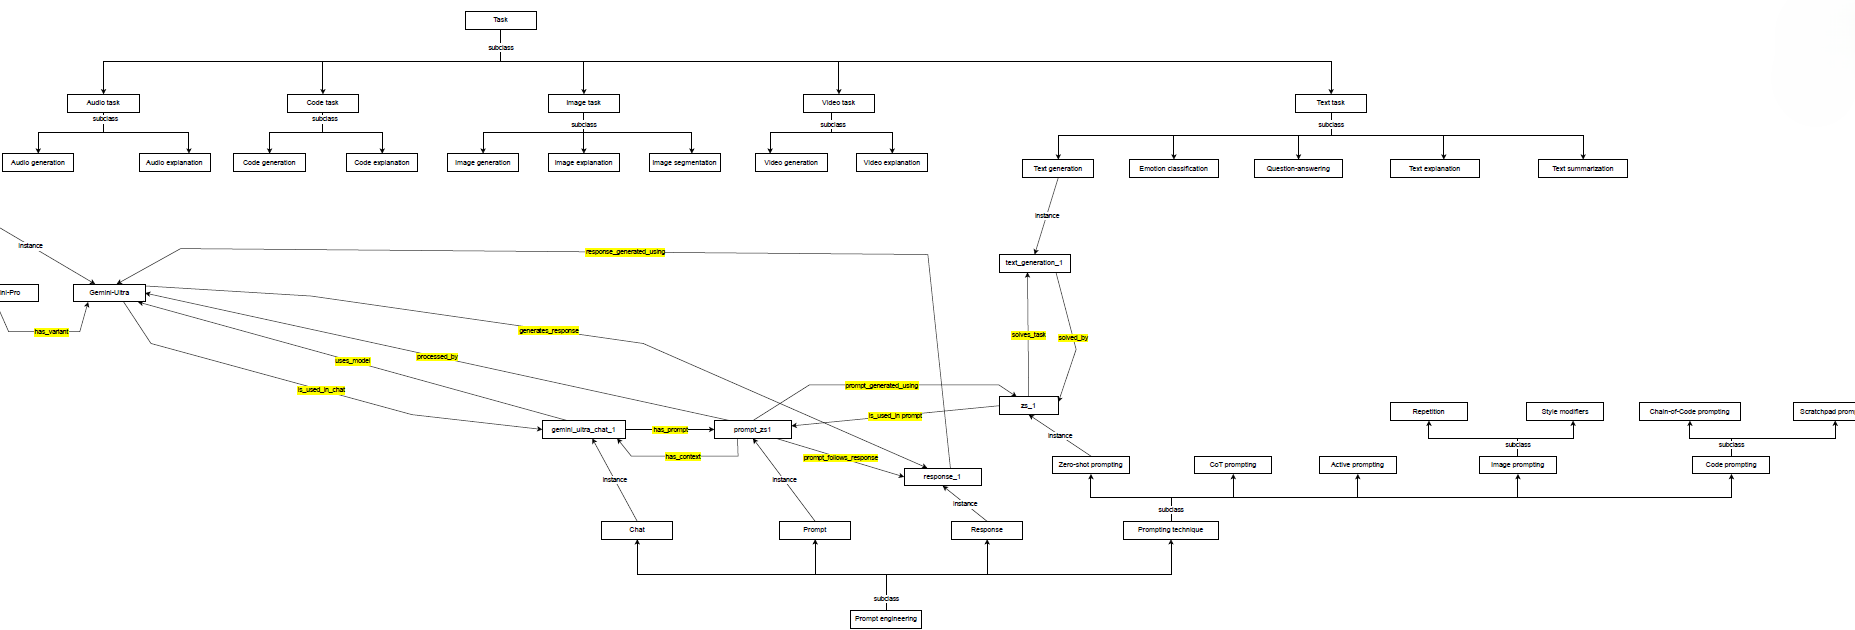
\includegraphics[width=0.9\linewidth]{Figures/fig_27.png}
    \caption{Prompt engineering\\ dimensions conceptualization}
    \label{fig:enter-label}
\end{figure}
After completing the conceptualization phase, the process can proceed to ontology reuse and ontology encoding. This involves first identifying similar ontologies within the domain of interest for potential reuse, followed by implementing and encoding the defined concepts using dedicated software tools.

\newpage
\section{Ontology reuse}
Before proceeding with ontology encoding, it is necessary to consider any similar ontologies that can be reused in the creation of the prompt engineering ontology. There are two types of reuse:
\begin{itemize}
    \item \textbf{Hard reuse:} it involves directly importing an entire ontology, rigidly incorporating it. Classes and properties are used without modification, ensuring semantic consistency but creating strong dependency on the original ontology.

    \item \textbf{Soft reuse:} it involves adapting or copying specific concepts without importing the complete ontology. This approach offers more flexibility, allowing customization, but it may introduce semantic inconsistencies or redundancies 
\end{itemize}

\subsection{Ontology design patterns reuse}


\subsection{State-of-art ontologies reuse}
I considered two ontologies that can be reused for the implementation of prompt engineering ontology:
\begin{enumerate}
    \item HALO ontology

    \item AI ontology
\end{enumerate}
The HALO ontology \cite{nananukul2024halo}, reviewed in the state-of-the-art chapter, has been considered due to its relevance to a domain closely connected to large language models, specifically addressing the hallucinations they generate. The ontology is accessible on \href{https://github.com/navapatn/halo-ontology}{Github} and despite the complete and exhaustive paper published, the published ontology is very poor. It has just twenty-five classes and non of them as an annotation or something to explain better the concept. There is a class called \textit{"LLMs Hallucination"} with two subclasses called \textit{"factuality hallucination"} and \textit{"faithfulness hallucination"} each one has subclasses about the type of hallucination that represent. Moreover there are pretty useless classes like \textit{"answers"} or \textit{"Book"} that seem have no sense in an ontology of this type, there are no individuals and just nine unused object properties. 
\begin{figure}[H]
    \centering
    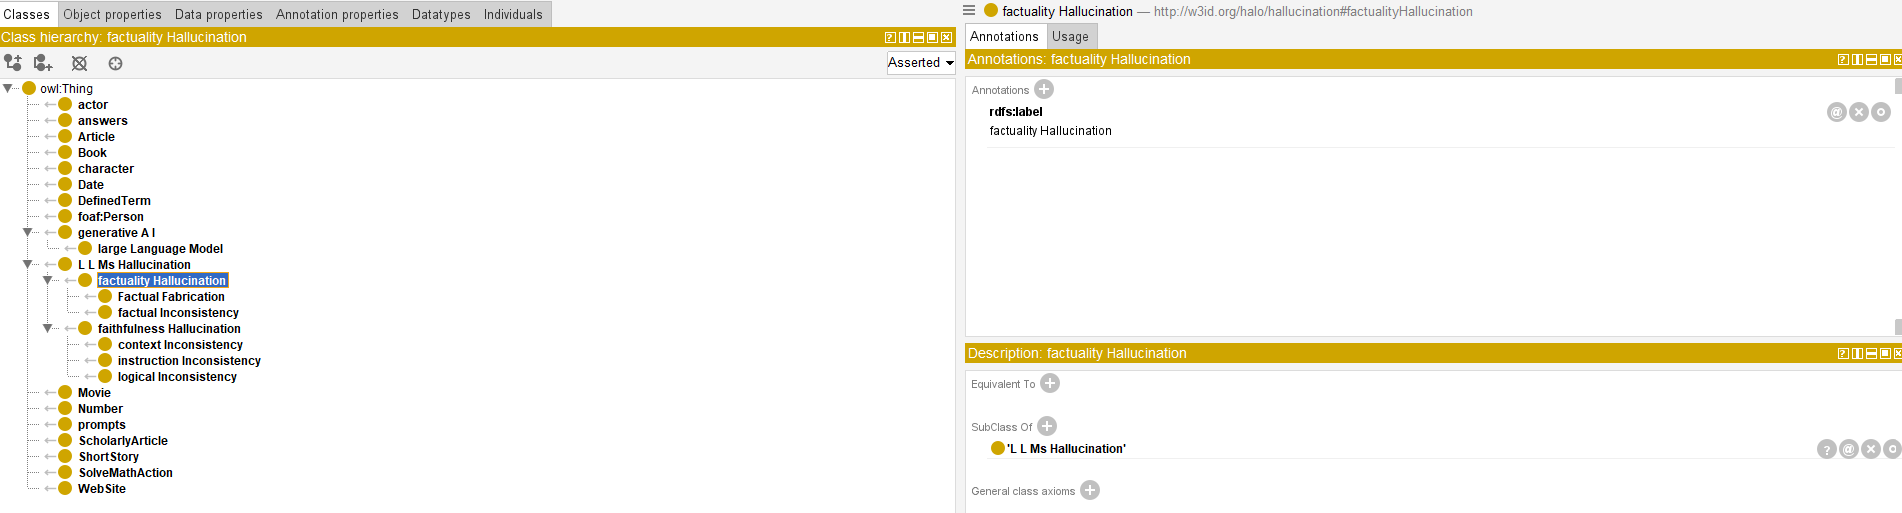
\includegraphics[width=1.0\linewidth]{Figures/fig_28.png}
    \caption{HALO ontology on Protegé}
    \label{fig:enter-label}
\end{figure}
This was sufficient to conclude that the HALO ontology would not be reused in the development of the prompt engineering ontology, as it would not offer any meaningful or valuable information.\\
The second ontology took into account is the Artificial Intelligence Ontology\cite{aio}, an ontology that covers machine learning methods, deep learning networks and their components. This ontology is particularly intriguing, as it stands out as one of the few, if not the only, ontologies focused on the field of artificial intelligence. The ontology is available on \href{https://github.com/berkeleybop/artificial-intelligence-ontology}{Github} in owl, json and csv format. Even in this case, despite the thorough study conducted, the ontology seems, in my opinion, incomplete in several aspects. Similar to the previous ontology, it includes only class labels without any additional annotations to clarify the represented concepts. The ontology is essentially a hierarchical structure, a taxonomy of concepts related to machine learning and deep learning, lacking both object properties and instances to populate the classes. The ontology, therefore, is not only useless in and of itself but, due to its lack of completeness, would not contribute any valuable information or serve as a meaningful reference for the prompt engineering ontology.\\ Prompt engineering and large language models represent a very recent field, and, as we have observed, only a few ontologies address it, often in a superficial and incomplete way. Therefore, I have chosen not to reuse any existing ontologies and to develop the prompt engineering ontology entirely from scratch. This approach allows me to represent the domain in the best possible way, without any limitations, and in a complete and clear manner.

\newpage
\section{Ontology encoding}
\subsection{Software in ontology encoding and the Protégé editor}
The ontology encoding phase is where the ontology is actually implemented. During this stage, the concepts and relationships defined in the conceptualization phase are formalized into a specific machine-readable language. Several tools are available to assist developers with this task. The main software tools for implementing ontologies include:
\begin{itemize}
    \item \href{https://protege.stanford.edu/}{Protégé}
    \item \href{https://www.cognitum.eu/semantics/fluenteditor/}{FluentEditor}
    \item \href{https://github.com/vivo-project/Vitro?tab=readme-ov-file}{Vitro}
    \item \href{https://www.semafora-systems.com/ontobroker-and-ontostudio-x}{OntoStudio}
\end{itemize}
To begin, I chose the software for my project and opted for \href{https://protege.stanford.edu/}{Protégé}: an open-source ontology editor developed by a team at Stanford University since 1987. Widely used and highly regarded among ontology engineers, it offers a user-friendly Eclipse-based interface and a wide range of features, including:
\begin{itemize}
    \item Ontology editing for OWL and RDF: it is possible to create, edit and visualize ontologies based on standard languages such as OWL (Web Ontology Language) and RDF (Resource Description Framework). 
    
    \item Reasoning and ontology validation: Protégé includes reasoning tools that allow the deduction of new information based on the rules defined in the ontology.

    \item Support for extensible plug-ins: Protégé supports a wide range of plug-ins, such as HermiT, FaCT++, and Pellet, which enhance reasoning, visualization, and ontology management capabilities.

    \item Ontology import and export: it is possible to import and export ontologies in various formats, including OWL, RDF/XML, Turtle, and JSON-LD, ensuring  compatibility with other tools and systems.

    \item Automatic documentation: Protégé supports the automatic creation of ontology documentation without any additional plug-in.

    \item SPARQL Query Support: Protégé allows users to execute SPARQL queries directly within the tool to extract specific information from the ontology.

    \item SWRL support: Protégé has the SWRL Tab which allows to define complex rules on concepts.
\end{itemize}
Only a limited number of ontology editors provide an extensive set of features tailored for developers. Moreover, several editors have remained outdated for years and suffer from lots of bugs. During the ontology development process, \href{https://git-scm.com/}{Git} was also used: a version control software to track changes made to the ontology changes that are synchronized with the \href{https://github.com/simonegramegna/peo}{GitHub repository}.
\subsection{Encoding beginning PEO ontology}
Starting from an empty page, the first thing to do is the definition of the ontology IRI (International Resource Identifier): which has to be unique and it has to refer to a standard organization. The ontology IRI of the PEO ontology is: \textit{https://w3id.org/peo\#}, this IRI will be in every entity created inside the ontology.
\begin{figure}[H]
    \centering
    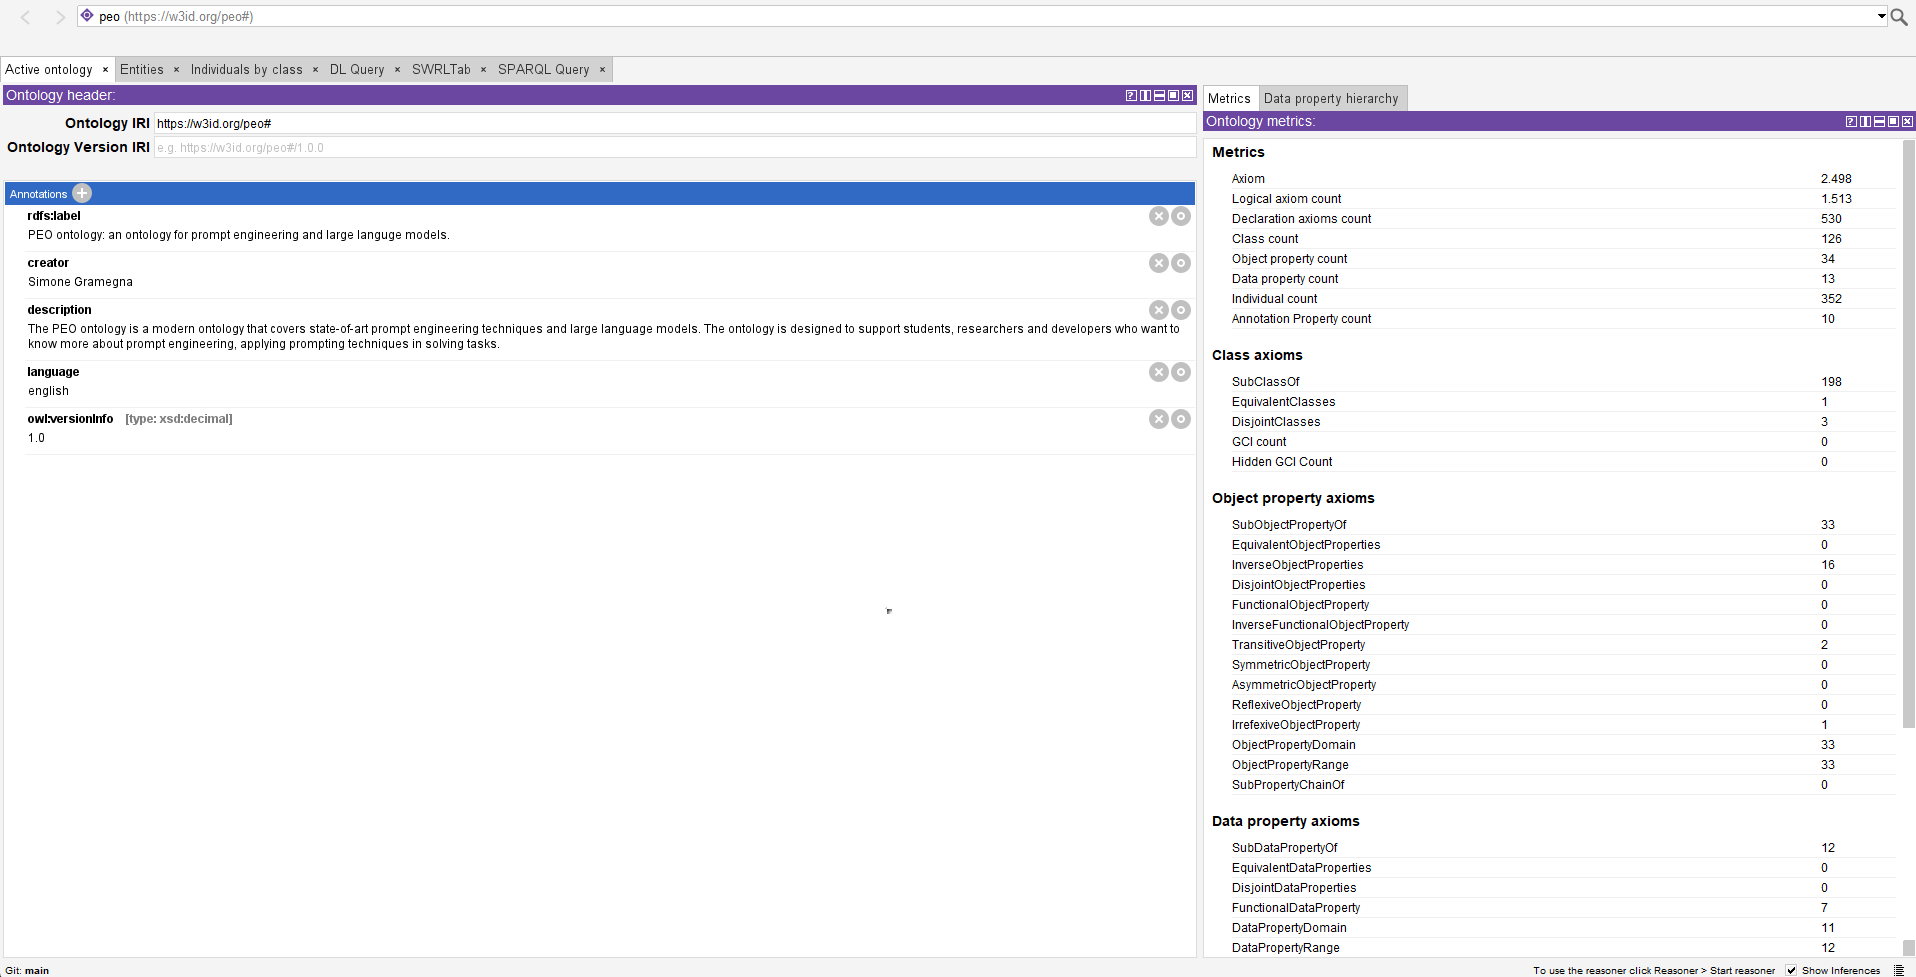
\includegraphics[width=0.8\linewidth]{Figures/fig_29.png}
    \caption{PEO ontology main page}
    \label{fig:enter-label}
\end{figure}
Once created the IRI, I defined the five annotations to properly describe the ontology:
\begin{table}[H]
    \centering
    \begin{tabular}{|>{\raggedright\arraybackslash}p{6cm}|>{\raggedright\arraybackslash}p{6cm}|}
        \hline
        \textbf{Annotation} & \textbf{Annotation value} \\ \hline
         rdfs:label & PEO ontology: an ontology for prompt 
         engineering and large language models. \\ \hline
         
         creator & Simone Gramegna\\ \hline
         
         rdfs:comment & The PEO ontology is a modern ontology that covers state-of-art prompt engineering techniques and large language models. The ontology is designed to support students, researchers and developers who want to know more about prompt engineering, applying prompting techniques in solving tasks. \\ \hline
         
         language & English \\ \hline
         
         owl:versionInfo & 1.0 \\ \hline
    \end{tabular}
    \caption{Ontology annotations in the main page}
\end{table}

Starting from the concepts outlined in the conceptualization phase, I define the primary classes of the ontology, which include:
\begin{itemize}
    \item \textbf{Base model}

    \item \textbf{Capability}

    \item \textbf{Large Language Model}

    \item \textbf{Organization}

    \item \textbf{Prompt engineering}

    \item \textbf{Task}
\end{itemize}
All these classes are mutually disjoint, as they represent distinct entities with no overlapping properties. The only exception is the relationship between "Base model" and "Capability", which are not disjoint. Both represent attributes of large language models and are collectively grouped under the \textbf{"LLM characteristic"} class, formed by the union of the two classes. \\
The Capability has five subclasses, each subclass has a label and a comment:
\begin{table}[H]
    \centering
    \begin{tabular}{|>{\raggedright\arraybackslash}p{6cm}|>{\raggedright\arraybackslash}p{6cm}|}
        \hline
        \textbf{Label} & \textbf{Comment} \\ \hline
         Audio processing &  Capability to process audio files. \\ \hline
         
         Code processing & Capability to process source code written in any programming language. \\ \hline
         
         Image processing & Capability to process images, understanding the content of the image. \\ \hline
         
         Text processing & Capability to process text and documents with text inside. \\ \hline
         
         Video processing & Capability to process video files. \\ \hline
    \end{tabular}
    \caption{Capability subclasses}
\end{table}
Each subclass has an individual with the same name, those individuals are created with the aim of assigning a capability to the instances of large language models that possess it, this aspect will be discussed later.

\subsection{Definition of large language models and characteristics}

The class "Base model" represents the models at the base of the architecture of large language models, it has six subclasses each one with label, description and reference and a subclass can have another subclass representing a more specific architecture, for example the subclass "Decoder" has inside the subclasses "Decoder only" and "Pixel decoder". 
I have included only the foundational models of the large language models represented in the ontology, excluding other base models as they fall outside the scope of this ontology. The subclasses included are: 
\begin{table}[H]
    \centering
    \begin{tabular}{|>{\raggedright\arraybackslash}p{6cm}|>{\raggedright\arraybackslash}p{6cm}|}
        \hline
        \textbf{Class} & \textbf{Subclasses} \\ \hline
         CLIP & none \\ \hline
         
         Decoder & Decoder-only, Pixel decoder \\ \hline
         
         Diffusion model & none \\ \hline
         
         Encoder & Encoder only, Global Image Encoder, Grounding Image Encoder, Region Encoder, ViT Encoder \\ \hline
         
         Recurrent Neural Network & none \\ \hline

        Transformer & Q-Former, LAMDA PT, Transformer XL \\ \hline
    \end{tabular}
    \caption{Base model subclasses}
\end{table}
The class "LLM characteristic" is subclass of both "Base model" and "Capability", each large language model subclass is connected to those two classes using the relations: \textit{has\_capability} (inverse relation \textit{is\_capability}) and\\ \textit{has\_model\_architecture}. In total there are 33 large language models subclasses of large language model, each subclass represents a type of a llm like GPT, Gemini ecc. The definition of large language models is completed with a label, a description, a link to the paper and a link to the website. Below there are large language models in the prompt engineering ontology with its own capability and architecture.
\begin{table}[H]
    \centering
    \begin{tabular}{|>{\raggedright\arraybackslash}p{4cm}|>{\raggedright\arraybackslash}p{4cm}|>{\raggedright\arraybackslash}p{4cm}|}
        \hline
        \textbf{LLM} & \textbf{Capability} & \textbf{Base model} \\ \hline
        Alpaca & Text processing & Transformer\\ \hline
        BERT & Text processing & Encoder only \\ \hline
        BLIP-2 & Image processing & Q-Former \\ \hline
        BLOOM & Text processing & Transformer \\ \hline
        Chinchilla & Text processing & Transformer \\ \hline
        Claude & Text processing & Transformer \\ \hline
        CogVLM & Image processing & ViT Encoder \\ \hline
        Command R & Text processing & Transformer \\ \hline
        DALL-E & Image processing & CLIP, Decoder, Transformer \\ \hline
        Falcon & Text processing & Decoder only \\ \hline
        FLAN & Text processing & LAMDA PT \\ \hline
        Gemini & Audio processing, Code processing, Image Processing, Text processing, Video processing & Transformer\\ \hline
        Gemma & Text processing & Transformer \\ \hline
    \end{tabular}
    \caption{Large language models in PEO ontology - part 1}
\end{table}

\begin{table}[H]
    \centering
    \begin{tabular}{|>{\raggedright\arraybackslash}p{4cm}|>{\raggedright\arraybackslash}p{4cm}|>{\raggedright\arraybackslash}p{4cm}|}
        \hline
        \textbf{LLM} & \textbf{Capability} & \textbf{Base model} \\ \hline
        GLaMM & Image processing & Global Image Encoder, Grounding Image Encoder \\ \hline
        LLaMA & Text processing & Transformer \\ \hline
        Midjourney & Image processing & Diffusion model  \\ \hline
        Minerva & Text processing & Transformer \\ \hline
        Mistral & Text processing & Transformer \\ \hline
        MPT-7B & Text processing & Decoder only \\ \hline
        OLMo & Text processing & Decoder only \\ \hline
        OpenELM & Text processing & Decoder only \\ \hline
        OPT & Text processing & Transformer \\ \hline
        PaLM & Text processing, Code processing & Transformer \\ \hline
        Phi-1 & Text processing & Transformer \\ \hline
        RWKV LLM & Text processing & Recurrent Neural Network, Transformer \\ \hline
        Sora & Video processing & Decoder only \\ \hline
        StableLM & Text processing & Decoder only \\ \hline
        StarCoder & Code processing & Decoder only \\ \hline
        T5 & Text processing & Transformer \\ \hline
        VALL-E & Audio processing & Transformer \\ \hline
        Vicuna & Text processing & Transformer \\ \hline
        XLNet & Text processing & Transformer XL \\ \hline
    \end{tabular}
    \caption{Large language models in PEO ontology - part 2}
\end{table}
There is a relation \textit{based\_on} between two subclasses of large language model (with inverse relation \textit{basis\_for}) where a large language model is developed starting from the base of another large language model. For example Alpaca is based on LLaMA (another family of large language models).\\
Each type of large language model has a capability, this capability is common for all instances of the large language model then if a specific version of a LLM has a new capability, the single LLM can be connected to that specific capability. For example GPT has capability text processing but GPT-3.5 has also the capability of code processing so this version has two capabilities (text processing and code processing). Same goes for GPT-4 which is an evolution of GPT-3.5 an it has the image processing capability, so it has three capabilities (text processing, code, processing and image processing). This approach is very flexible an efficient because there is no need to divide into categorical classes each version of large language model by simply connecting the version with the specific instance oof the capability. There are three relations between versions of the same large language model: 
\begin{itemize}
    \item \textit{has\_variant:} relation between two large language models (x and y), where x has y as another version.

    \item \textit{evolves:} transitive relation between two large language models (x and y), where y is an evolution of x. 

    \item \textit{evolved\_from:} transitive inverse relation of \textit{evolves} between two large language models x and y.
\end{itemize}
While the relation \textit{has\_variant} does not express an evolution but just a different version of the model, the relation \textit{evolves} implies also the relation \textit{has\_variant}, for example if GPT-3.5 evolves GPT-4 then GPT-3.5 has variant GPT-4, this cannot be expressed using relation but using SWRL rules. SWRL rules are are logical expressions that extend OWL ontologies by allowing the definition of conditional "if-then" rules for reasoning, those rules are processed by a reasoner during the inference. The chosed reasoner is the Hermit reasoner\cite{glimm2014hermit}: a reasoner already included in Protégé which does not require the installation of any additional plug-in. The reasoner ensures the ontology consistency, inferring new axioms and processing SWRL rules. SWRL rules are widely applied in the ontology, the first application is the creation of a new relation \textit{has\_variant} if there is the \textit{evolves} relation, the rule is expressed in this way:
\begin{lstlisting}
peo:evolves(?x, ?y) -> peo:has_variant(?x, ?y)
\end{lstlisting}
$?x$ and $?y$ express the two instances involved in the relations and the rules is applied to all instances that satisfy the condition in the body of the rule. If a model evolves into another model, the evolved model has the capabilities of the previous model, this concept is expressed using this SWRL rule:
\begin{lstlisting}
peo:evolves(?x, ?y) ^ peo:has_capability(?x, ?c) -> peo:has_capability(?y, ?c)
\end{lstlisting}
These two relations are not explicitly defined in the ontology but are inferred by the reasoner during the reasoning process, making them visible at that stage.
Each instance of large language model has two data properties associated 
\begin{itemize}
    \item \textit{has\_number\_parameters:} number of parameters of the model.

    \item \textit{has\_release\_year:} year of release of the model
\end{itemize}
Those two data properties are functional, assigning a single value of each property to the instance of the llm.\\
Large language models are developed by organizations that can be universities, research institutions and companies for business purpose, the class \textbf{Organization} contains those three subclasses (with label  and description) and each subclass has instances representing the specific organization.
\begin{table}[H]
    \centering
    \begin{tabular}{|>{\raggedright\arraybackslash}p{6cm}|>{\raggedright\arraybackslash}p{6cm}|}
        \hline
        \textbf{Subclass or organization} & \textbf{Number of entities} \\ \hline
        
        University & 2 \\ \hline
 
        Research institution & 8 \\ \hline
        
        Company & 13 \\ \hline
    \end{tabular}
    \caption{Number of organization entities}
\end{table}
Every instance of organization has two associated data properties:
\begin{itemize}
    \item \textit{registered\_name:} the official name of the organization.

    \item \textit{official\_website:} the official website of the organization.
\end{itemize}
Organization instances and large language models are connected using the \textit{develops} relation, connecting an instance of organization with an instance of large language models. We well know that an organization does not develop a single version of an LLM but the entire family (represented by the different subclasses of the large language model class) but it is not possible to have a relation between an instance and a subclass. A possible solution could be putting manually the develops relation between the company and all version developed but it would be too long. Instead of doing this process, using the \textit{has\_variant} relation previously defined, I created the following SWRL rule:
\begin{lstlisting}
peo:develops(?c, ?x) ^ peo:has_variant(?x, ?y) -> peo:develops(?c, ?y)    
\end{lstlisting}
If a company $c$ develops a large language model $?x$ and the large language model $x$ has variant another large language model (of the same type) $y$ then the company $c$ develops the llm $y$. This rule requires that the relationship \textit{has\_variant} exists among all versions of large language models or the relation \textit{evolves} should exist, in order to infer \textit{has\_variant}. For example if OpenAI develops GPT-1, GPT-1 evolves GPT-2 (has variant GPT-2) then OpenAI develops GPT-2. This process during the inference is automatic because the \textit{evolves} relation is transitive. Another SWRL rule that involves the \textit{develops} relation is the following:
\begin{lstlisting}
peo:is_organization_of(?o1, ?o2) ^ peo:develops(?o1, ?llm) -> peo:develops(?o2, ?llm)
\end{lstlisting}
If an organization $o1$ is organization of another organization $o2$ (for example DeepMind is organization of Google) and $o1$ develops a large language model then $o2$ develops the llm. This was important to specify because different researchers teams rely on other organization that finance them and provide them with resources.

\subsection{Definition of task}
The \textbf{Task} class represents task that are solved by large language models applying prompting techniques, there are five specific subclasses representing the different types of task distinguished based on the type of data to process: image, text, video, audio, or code. Each subclass has other subclasses representing the specific task for example audio generation, text translation ecc as we can see in the table below:
\begin{table}[H]
    \centering
    \begin{tabular}{|>{\raggedright\arraybackslash}p{6cm}|>{\raggedright\arraybackslash}p{6cm}|}
        \hline
        \textbf{Task type} & \textbf{Subclasses} \\ \hline
        Audio task & Audio generation, Audio explanation \\ \hline

        Video task & Video generation, Video explanation \\ \hline
    \end{tabular}
    \caption{Types of task with subclasses - part 1}
\end{table}

\begin{table}[H]
    \centering
    \begin{tabular}{|>{\raggedright\arraybackslash}p{6cm}|>{\raggedright\arraybackslash}p{6cm}|}
        \hline
        \textbf{Task type} & \textbf{Subclasses} \\ \hline
        Code task & Code generation, Code explanation \\ \hline

        Image task & Image generation, Image explanation, Image segmentation \\ \hline

        Text task & Emotion classification, Mathematical understanding, Question-Answering, Text explanation, Test generation, Text summarization, Text translation \\ \hline
    \end{tabular}
    \caption{Types of task with subclasses - part 2}
\end{table}
All of those classes have a label and a description describing shortly the task and they can have one or more instances, each instance represents a specific task of that type, it has a data property called \textit{has\_description} to specify the description of the task.

\subsection{Definition of prompt engineering}
The \textbf{Prompt engineering} class includes all concepts associated with prompts, such as their creation, the context in which they are applied, and the responses they produce. It has four main subclasses, each one with a label and a description:
\begin{itemize}
    \item \textbf{Chat:} context in which a prompt is created. 
    \item \textbf{Prompt:} input to a large language model.
    \item \textbf{Prompting technique:} technique used to create a prompt.
    \item \textbf{Response:} response given by a large language model after a prompt.
\end{itemize}
The prompting technique is very important because it has all the subclasses representing the different prompting techniques and all instances of those classes are connected using different object properties. All subclasses of Prompting Technique refer to techniques used in tasks that involve processing only textual content. Prompting techniques related to images and source code are specifically addressed by their respective subclasses \textbf{Code prompting technique} and \textbf{Image prompting techniques}, each subclass has subclasses with specific techniques. Prompting techniques for audio and video have not been specified, as the few existing techniques are experimental and not yet well-established. Moreover, for obvious reasons, they would be challenging to represent within the ontology. The prompting techniques are gathered from papers, as seen in the background chapter, each subclass representing the specific technique has a label, a description and a reference. In total there are 24 prompting techniques:
\begin{itemize}
    \item Active prompting
    \item Analogical prompting
    \item Automatic Chain-of-Thought prompting
    \item Chain-of-Knowledge prompting
    \item Chain-of-Note prompting
    \item Chain-of-Table prompting
    \item Chain-of-Thought prompting
    \item Chain-of-Verification prompting
    \item Decomposed prompting
    \item Emotion prompting
    \item Few shot prompting
    \item Graph of Thoughts prompting
    \item Least-to-most prompting
    \item Logical Chain-of-Thought prompting
    \item ReAct prompting
    \item Retrieval Augmented Generation - RAG prompting
    \item Role prompting
    \item Self consistency prompting
    \item System-2-Attention prompting
    \item Take a step back prompting
    \item Thread of Thought prompting
    \item Tree of Thoughts prompting
    \item Zero shot prompting
\end{itemize}
For code, the class Code Prompting Technique has four subclasses:
\begin{itemize}
    \item Chain-of-Code prompting
    \item Program of Thoughts prompting
    \item Scratchpad prompting
    \item Structured Chain-of-Thought prompting
\end{itemize}
Image prompting technique class has six subclasses:
\begin{itemize}
    \item Fix deformed generations prompting
    \item Lighting
    \item Quality boosters
    \item Repetition
    \item Shot type
    \item Style modifiers
\end{itemize}
To ensure the accurate and consistent representation of prompts generated using the listed techniques, instances of the Prompting Technique class are connected to instances of other Prompt Engineering subclasses via dedicated object properties, defined explicitly or inferred by the reasoner using SWRL rules. To illustrate all instances along with their associated object properties and data properties, I propose a simple task: translating the phrase \textit{"Ciao, come va?"} from Italian to English using a zero-shot prompt as input to GPT-4.\\
The first step is to create, if it does not already exist, an instance of the "Text translation" subclass of Task, which we will name \textit{"translation\_1"} assigning the data property \textit{has\_description} the string value: \textit{"Translation of the text: Ciao, come va?"}. Now I create the instance of the prompting technique that is going to solve the task, in this case we create an instance of the subclass "Zero shot prompting" called \textit{"zs\_prompting\_1"}. This instance is connected to \textit{"translation\_1"} using the object property \textit{solves\_task} with the inverse property \textit{"solved\_by"} connecting the two instances in both directions. Before creating the prompt, we create an instance of the chat class, calling it \textit{"gpt4\_chat\_1"} and connecting to the instance \textit{GPT-4} of the GPT class using the object property \textit{uses\_model} with inverse property \textit{is\_used\_in\_chat}. The chat instance has three data properties associated:
\begin{itemize}
    \item \textit{has\_chat\_title:} title of the chat, I assign it "Translation GPT-4 italian to english 1".

    \item \textit{start\_time\_chat:} start time of the chat, I assign to it the currant time while I'm writing this chapter: "29/11/2024 - 10:37"

    \item \textit{end\_time\_chat:} end time of the chat, the chat has the duration of two minutes and I assign the value: "29/11/2024 - 10:39"
\end{itemize}
Obviously those values assigned without any criteria can be modified later. Now that a context is established, the chat \textit{"gpt4\_chat\_1"}, I proceed to create the instance of the Prompt. I specify that the prompt called \textit{"zs\_1"} is created using the instance of Zero shot prompting previously defined using the object property \textit{prompt\_generated\_using} with inverse property \textit{is\_used\_in\_prompt}, in our case \textit{"zs\_1"} is generated using \textit{"zs\_prompting\_1"}. A prompt instance can have three associated data properties:
\begin{itemize}
    \item \textit{has\_instruction:} main instruction of the prompt.

    \item \textit{has\_input\_data:} data given as input to the prompt. 

    \item \textit{has\_output\_indicator:} indicator that indicates the format of the response.
\end{itemize}
For simplicity, I assign only the instruction \textit{"Translate the English text to Italian. Text: Ciao, come va? Translation:"} to the prompt, other data properties values can be added later. Now I connect the prompt with its context, the \textit{"gpt4\_chat\_1"} using the object property \textit{has\_context} with inverse relation \textit{has\_prompt} and after the creation of this relation using an SWRL rule I connect the prompt with the large language model that takes it in input. 
\begin{lstlisting}
peo:has_context(?p, ?c) ^ peo:uses_model(?c, ?m) -> peo:processed_by(?p, ?m)   
\end{lstlisting}
If a prompt $?p$ has a context the chat $?c$ and it uses the model $?m$ then $?p$ is processed by the model $?m$. This rule creates automatically during the reasoning the relation \textit{processed\_by} with inverse relation \textit{processes}. After a prompt, the llm generates a response, in PEO ontology is instance of the Response class, the value is associated using the data property \textit{has\_response\_value} and it is connected to the prompt that generated it using the object property \textit{response\_followedby\_prompt}. In order to model the "chain" prompt-responses-prompt I created the following object properties:
\begin{itemize}
    \item \textit{response\_followedby\_prompt:} the response is after a prompt.

    \item \textit{prompt\_follows\_response:} after the prompt there is a response, inverse property of \textit{response\_followedby\_prompt}.

    \item \textit{prompt\_follows\_prompt:} after the prompt there is another prompt.

    \item \textit{prompt\_followedby\_prompt:} before the prompt there is another prompt, inverse property of {prompt\_follows\_prompt}.

    \item \textit{response\_follows\_prompt:} after the response there is a prompt.

    \item \textit{prompt\_followedby\_response:} before the prompt there is a response, inverse relation of \textit{response\_follows\_prompt}. 
\end{itemize}
We can graphically see this concatenation in the following scheme:
\begin{figure}[H]
    \centering
    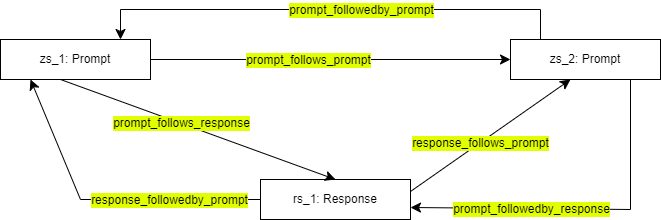
\includegraphics[width=0.9\linewidth]{Figures/fig_30.png}
    \caption{Chain prompt-response}
    \label{fig:enter-label}
\end{figure}
Of course, most of these relationships are automatically created during the inference process. To connect a response with the next prompt, I created this SWRL rule:
\begin{lstlisting}
peo:prompt_followedby_prompt(?x, ?y) ^ peo:prompt_follows_response(?y, ?r) -> peo:prompt_followedby_response(?x, ?r)
\end{lstlisting}
If a prompt $?x$ is followed by another prompt $?y$ and $?y$ has a response $?r$ then $?x$ is followed by $?r$. The context next prompt is assigned automatically using the object property \textit{prompt\_followedby\_prompt} ant this SWRL rule:
\begin{lstlisting}
peo:prompt_followedby_prompt(?x, ?y) ^ peo:has_context(?y, ?c) -> peo:has_context(?x, ?c)
\end{lstlisting}
If a prompt $x$ is followed by another prompt $y$ and $y$ has context the chat $c$ then $x$ has context $c$. Also each response is connected the chat using the object property \textit{is\_response\_of} (inverse property \textit{has\_response}) created using the SWRL rule:
\begin{lstlisting}
peo:response_followedby_prompt(?r, ?p) ^ peo:has_context(?p, ?c) -> peo:is_response_of(?r, ?c)
\end{lstlisting}
If a response $?r$ is followed by a prompt $?p$ and the prompt $?p$ has the context the chat $?c$ then the response $?r$ is response of $?c$. The last SWRL rule connects the response with the model that has generated it creating the object property \textit{response\_generated\_using} with inverse property \textit{generates\_response}:
\begin{lstlisting}
peo:response_followedby_prompt(?r, ?p) ^ peo:processed_by(?p, ?m) -> peo:response_generated_using(?r, ?m) 
\end{lstlisting}
If a response $?r$ is followed by a prompt $?p$ and the prompt $?p$ is processed by the large language model $?m$ then the response $?r$ is generated using $?m$.\\
All these object properties may seem unclear so below is a diagram that shows all the relationships involved in creating a chat.
\begin{figure}[H]
    \centering
    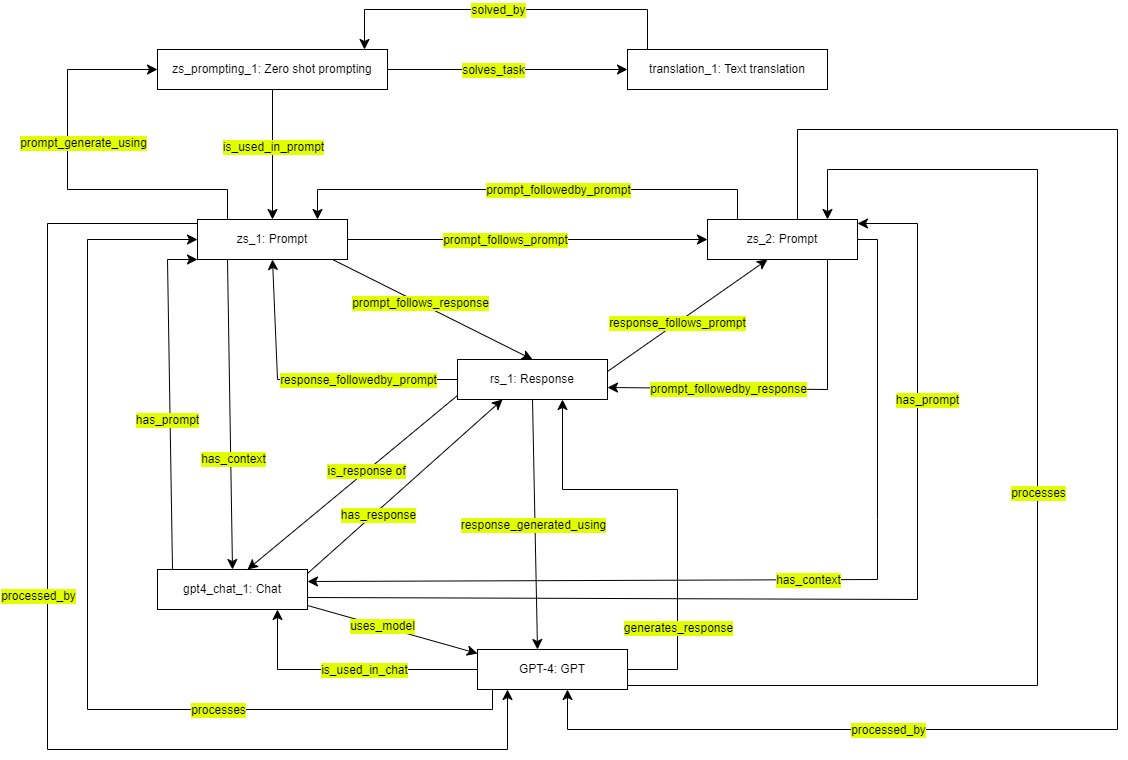
\includegraphics[width=0.85\linewidth]{Figures/fig_31.png}
    \caption{Chat scheme}
    \label{fig:enter-label}
\end{figure}


\subsection{Ontology population with prompts}
Populating the ontology with prompts is a complex process as it requires connecting various instances (task, prompting technique, prompt, chat, response, large language model) using the defined object properties. Moreover, each prompt is manually crafted in accordance with the specific prompting technique. Manually populating the ontology with all instances for every task, every version of each large language model, and every prompting technique would be highly time-consuming and beyond the objectives of this thesis. Therefore, a decision was made to populate only a specific subset of the ontology choosing large language model versions, tasks and prompting techniques. Large language models chosed are very popular LLM available to the users and they are represented in the ontology:
\begin{itemize}
    \item \textbf{GPT-4}
    \item \textbf{Mistral-7B}
    \item \textbf{Gemini Flash}
\end{itemize}
Then I chosed five prompting techniques with a criterium for each one:
\begin{itemize}
    \item \textbf{Zero-shot prompting:} this technique allows large language models to handle new tasks using only natural language instructions, without requiring examples or any effort by the user.

    \item \textbf{Few-shot prompting:} this technique  enables language models to learn new tasks with few examples, reducing the need for extensive task-specific datasets.
    
    \item \textbf{Role prompting:} this technique improves large language models performance on solving tasks by simulating specific roles.

    \item \textbf{Emotion prompting:} this technique enhances large language models by integrating emotions into prompts, improving response generation and performance on tasks.

    \item \textbf{Analogical prompting:} this technique is able to generate automatically task-specific exemplars, reducing manual annotation needs, and improving performance on problem-solving tasks.
\end{itemize}
Finally I chosed four task to solve applying prompting techniques and using large language models defined:
\begin{itemize}
    \item \textbf{Emotion classification:} classification of the emotion in a given text.

    \item \textbf{Mathematical understanding:} solving a given mathematical problem of medium difficulty. 

    \item \textbf{Text translation:} translation of a text from english to italian.

    \item \textbf{Text summarization:} summarization of the content of a given text.
\end{itemize}
Below, I list the prompts created for each task.\\\\
\textbf{Task 1: Emotion classification}\\     
The text to classify the emotion is: \textit{"I think the vacation is okay"}
\begin{itemize}
    \item \textbf{Zero-shot prompting:} Classify the text into neutral, negative or positive. Text: "I think the vacation is okay." Sentiment:
    \item \textbf{Few-shot prompting:} Classify the following text into neutral, negative, or positive based on its sentiment. Here are some examples: 
    Text: "The food was absolutely wonderful!" Sentiment: Positive. 
    Text: "I did not enjoy the movie at all." Sentiment: Negative. 
    Text: "It was an average experience." Sentiment: Neutral. 
    Now, classify this text: Text: "I think the vacation is okay." Sentiment:
    \item \textbf{Emotion prompting:} Classify the following text into neutral, negative, or positive based on its sentiment. This task is very important to my career. Please provide a well-thought and accurate classification. Text: "I think the vacation is okay." Sentiment:
    \item \textbf{Role prompting:} From now on, you are an experienced sentiment analyst with deep expertise in understanding human emotions through textual analysis. Your task is to classify the sentiment of texts as neutral, negative, or positive with utmost accuracy and professionalism. Text: "I think the vacation is okay." Sentiment:
    \item \textbf{Analogical prompting:} Classify the text into neutral, negative or positive. \# Instruction: \# Text: I think the vacation is okay. \# Sentiment:
\end{itemize}
\textbf{Task 2: Mathematical understanding}\\
For the mathematical understanding there is the solving of a simple geometrical problem: the calculation of a square with the four vertices at (-2, 2), (2, -2), (-2, -6), and (-6, -2). 
\begin{itemize}
    \item \textbf{Zero-shot prompting:} What is the area of the square with the four vertices at $(-2, 2)$, $(2, -2)$, $(-2, -6)$, and $(-6, -2)$?
    \item \textbf{Few-shot prompting:} Instruction: Determine the area of a square given the coordinates of its four vertices. 
    Example 1: Vertices: $(0, 0)$, $(4, 0)$, $(4, 4)$, $(0, 4)$ 
    Step 1: Identify the side length. Distance between $(0, 0)$ and $(4, 0)$ is $\sqrt{((4 - 0)^2 + (0 - 0)^2)} = 4$. 
    Step 2: Calculate the area. Area = side length$^2 = 4^2 = 16$. Answer: 16. 
    Example 2: Vertices: $(-1, 1)$, $(-1, 3)$, $(1, 3)$, $(1, 1)$ 
    Step 1: Identify the side length. Distance between $(-1, 1)$ and $(-1, 3)$ is $\sqrt{((3 - 1)^2 + (1 - 1)^2)} = 2$. 
    Step 2: Calculate the area. Area = side length$^2 = 2^2 = 4$. Answer: 4. 
    Query: Vertices: $(-2, 2)$, $(2, -2)$, $(-2, -6)$, $(-6, -2)$. 
    Step 1: Identify the side length by calculating the distance between consecutive vertices. 
    Step 2: Calculate the area of the square. Answer:
    \item \textbf{Emotion prompting:} Please calculate the area of a square given the coordinates of its vertices. This task is important for building my understanding of geometry and improving my analytical skills, so I truly value a thorough and accurate solution. Vertices: $(-2, 2)$, $(2, -2)$, $(-2, -6)$, $(-6, -2)$.
    \item \textbf{Role prompting:} From now on, you are a brilliant geometry teacher. You always explain geometry problems thoroughly and ensure your students understand every step of the process. I have a question for you: I have four vertices of a square: $(-2, 2)$, $(2, -2)$, $(-2, -6)$, and $(-6, -2)$. Can you help me calculate the area of the square step by step? Please provide a detailed explanation of how to verify the shape, calculate the side length, and determine the area.
    \item \textbf{Analogical prompting:} What is the area of the square with the four vertices at $(-2, 2)$, $(2, -2)$, $(-2, -6)$, and $(-6, -2)$? \# Instruction: \#\# Recall relevant exemplars: \#\# Solve the initial problem:
\end{itemize}
\textbf{Task 3: Text translation}\\
For text translation task I chosed a citation of Lewis Carol \cite{carol} to translate form english to italian: \textit{"Sometimes, I've believed as many as six impossible things before breakfast."}
\begin{itemize}
    \item \textbf{Zero-shot prompting:} Translate the English text to Italian. Text: "Sometimes, I've believed as many as six impossible things before breakfast." Translation:
    \item \textbf{Few-shot prompting:} Translate the following English sentences into Italian: 
    1. English: "Sometimes, I've believed as many as six impossible things before breakfast." Italian: "A volte, ho creduto a ben sei cose impossibili prima di colazione." 
    2. English: "I think, therefore I am." Italian: "Penso, quindi sono." 
    3. English: "All the world's a stage, and all the men and women merely players." Italian: "Tutto il mondo è un palcoscenico e tutti gli uomini e le donne sono solo attori." 
    Now translate this sentence: English: "Sometimes, I've believed as many as six impossible things before breakfast." Italian:
    \item \textbf{Emotion prompting:} Translate the following text to Italian. It's very important for me to understand this translation accurately as it could affect my professional progress: "Sometimes, I've believed as many as six impossible things before breakfast."
    \item \textbf{Role prompting:} From now on, you are an excellent literary translation teacher who accurately explains the meaning and tone of complex sentences. Translate the following sentence from English to Italian, preserving its meaning and tone: "Sometimes, I've believed as many as six impossible things before breakfast."
    \item \textbf{Analogical prompting:} \# Problem: "Sometimes, I've believed as many as six impossible things before breakfast." 
    \# Relevant Problems: 
    1. Translating a complex sentence from English to Italian. 
    - Question: How to translate the sentence "To be or not to be, that is the question" into Italian? 
    - Answer: The sentence "To be or not to be, that is the question" translates into Italian as "Essere o non essere, questo è il problema." 
    2. Translating a sentence with idiomatic expressions. 
    - Question: How to translate "Break a leg!" into Italian? 
    - Answer: The idiomatic expression "Break a leg!" translates into Italian as "In bocca al lupo!" 
    3. Translating a sentence with abstract concepts. 
    - Question: How to translate "The only limit is your imagination" into Italian? 
    - Answer: The sentence "The only limit is your imagination" translates into Italian as "L'unico limite è la tua immaginazione." 
    \# Translation of the initial problem: The sentence "Sometimes, I've believed as many as six impossible things before breakfast" translates into Italian as:
\end{itemize}
\textbf{Task 4: Text summarization}\\
The last task is the summarization of the following text about permaculture: \textit{"Permaculture is a design process mimicking the diversity, functionality and resilience of natural ecosystems. The principles and practices are drawn from traditional ecological knowledge of indigenous cultures combined with modern scientific understanding and technological innovations. Permaculture design provides a framework helping individuals and communities develop innovative, creative and effective strategies for meeting basic needs while preparing for and mitigating the projected impacts of climate change."}\cite{permaculture}
\begin{itemize}
    \item \textbf{Zero-shot prompting:} Permaculture is a design process mimicking the diversity, functionality and resilience of natural ecosystems. The principles and practices are drawn from traditional ecological knowledge of indigenous cultures combined with modern scientific understanding and technological innovations. Permaculture design provides a framework helping individuals and communities develop innovative, creative and effective strategies for meeting basic needs while preparing for and mitigating the projected impacts of climate change. Write a summary of the above text. Summary:
    \item \textbf{Few-shot prompting:} You are an expert at creating concise summaries. Below are some examples of summaries based on texts.
    Example 1: Text: The Earth orbits the Sun in an elliptical pattern, taking approximately 365.25 days to complete one orbit. This forms the basis of the Gregorian calendar year. Summary: The Earth completes an orbit around the Sun in roughly 365 days, defining the calendar year.
    Example 2: Text: Sustainable agriculture incorporates practices that maintain productivity and minimize environmental impact, such as crop rotation and organic farming. Summary: Sustainable agriculture uses eco-friendly practices like crop rotation and organic methods to maintain productivity.
    Task: Text: Permaculture is a design process mimicking the diversity, functionality, and resilience of natural ecosystems. The principles and practices are drawn from traditional ecological knowledge of indigenous cultures combined with modern scientific understanding and technological innovations. Permaculture design provides a framework helping individuals and communities develop innovative, creative, and effective strategies for meeting basic needs while preparing for and mitigating the projected impacts of climate change. Summary:
    \item \textbf{Emotion prompting:} Summarize the essence of permaculture, focusing on its innovative design process inspired by natural ecosystems. Highlight how it combines traditional ecological knowledge with modern science and technology to address climate change. This understanding is vital to my research and the future of sustainable living. Please ensure the summary is concise yet comprehensive.
    \item \textbf{Role prompting:} From now on, you are an environmental scientist who specializes in explaining complex ecological concepts in an accessible and engaging manner. Your task is to provide a concise summary of permaculture principles and their importance in addressing climate challenges.
    \item \textbf{Analogical prompting:} Problem: Summarize the definition and essence of permaculture using principles that mirror natural ecosystems and combine traditional ecological knowledge with modern science. Instruction: Recall three relevant and distinct problems or topics related to summarizing processes that focus on mimicking complex systems. Provide detailed exemplars for each recalled instance, including how the principles were extracted and utilized effectively. Use the recalled insights to structure and write the final summary.
\end{itemize}
The responses for each prompt from the three large language models have been saved in the ontology, and a chat has been created for each prompt, including a title, start time, and end time resulting in a total of 60 distinct chats.
\begin{figure}[H]
    \centering
    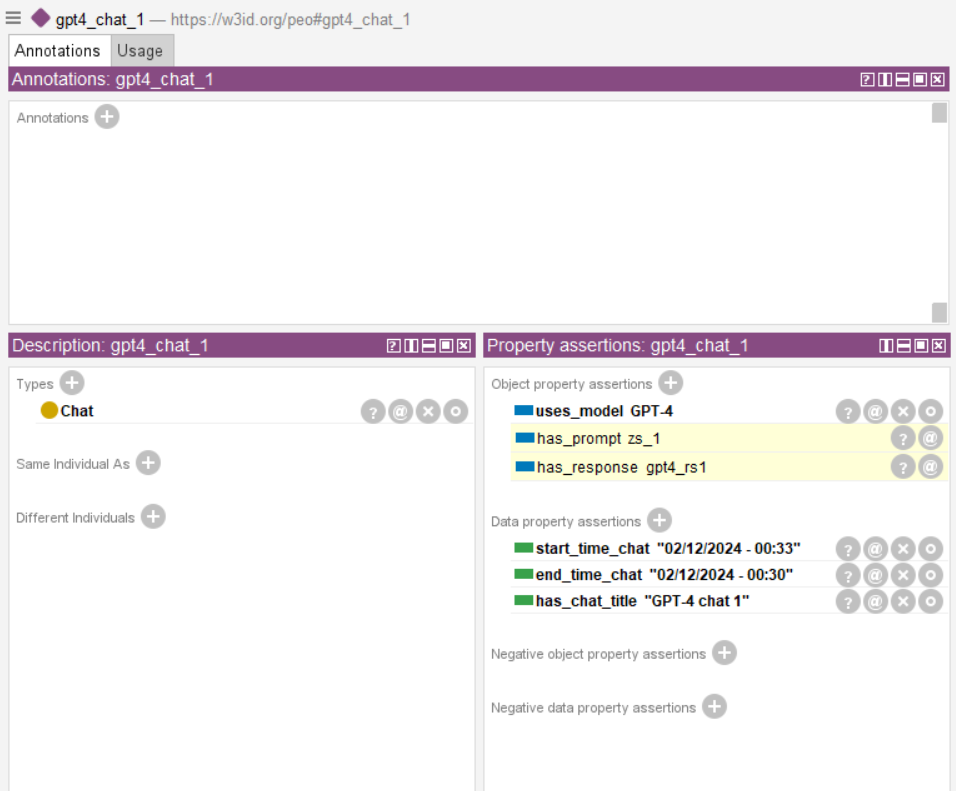
\includegraphics[width=0.75\linewidth]{Figures/fig_32.png}
    \caption{Example of chat with relations inferred}
    \label{fig:enter-label}
\end{figure}

\subsection{Automatic ontology population}
Populating an ontology with various instances can be a time-consuming task for developers, as the ontology's domain of interest often involves numerous entities requiring manual insertion. To streamline this process and reduce the developer's effort, automation can be employed. There are different researches dedicated to the automatic population of ontologies, one of the most recent is \textit{"Ontology Population using LLMs"} \cite{norouzi2024ontology}, it proposes a methodology to semi-automatically populate modular ontologies using Large Language Models (LLMs). It focuses on leveraging the strengths of LLMs, such as GPT-4 and Llama-3, for extracting structured knowledge from natural language texts. The method is divided into three main stages: data preprocessing, relevant text retrieval, and ontology population. In the first stage, the data is cleaned, organized, and aligned with simplified ontology modules to facilitate processing. The second stage employs text summarization and Retrieval-Augmented Generation (RAG) techniques to identify and extract relevant information aligned with the ontology schema. Finally, in the third stage, predefined module files guide the LLMs to populate the ontology with accurate triples by using structured prompts. Despite the good results, the methodology still requires effort, as documents need to be selected and preprocessed to create a dataset that serves as input for the large language model used to populate the ontology. Implementing this process demands skills that go beyond those of an ontology engineer, effectively shifting the workload to another task.\\ 
Another approach is proposed in the paper \textit{"Financial Product Ontology Population with Large Language Models"} \cite{saetia2024financial}, it leverages Large Language Models (LLMs), such as GPT-3.5 and GPT-4, to populate financial ontologies by extracting structured data from unstructured texts. It combines several prompting techniques to improve accuracy and scalability. Few-shot prompting provides positive and negative examples to guide the model's understanding. Chain-of-Thought (CoT) reasoning encourages sequential reasoning, while schema.org definitions are included to contextualize fields and properties. Prompts are carefully designed to generate structured outputs in JSON format for easy integration and evaluating performance using F1 scores, with the best results achieved when combining examples, CoT, and definitions. Like the previous one, this approach requires a lot of job on gathering necessary docs to pre-process and this process can be time-consuming, also the quality of the output depends on the prompts.\\ These tasks divert attention from the main objective and increase the developer's workload. Rather than using the methodologies outlined in the literature, I opted for a more straightforward and pragmatic approach to populating the ontology. Starting from the sixteen competency questions defined in the \textit{Ontology requirements specification} section, I input them, together with the ontology, into a large language model to generate an automatically populated version of the prompt engineering ontology. The large language model chosed is GPT-4o: the latest and most powerful version of GPT available in its web interface \href{https://chatgpt.com/}{ChatGPT} and used previously in the manual ontology population. This time instead of giving as input a specific prompt created with one of prompt engineering techniques, I write this prompt, providing the ontology and a text file containing the competency questions.
\begin{figure}[H]
    \centering
    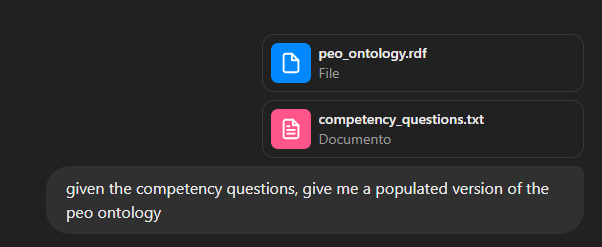
\includegraphics[width=0.9\linewidth]{Figures/fig_34.png}
    \caption{Prompt for automatic ontology population}
    \label{fig:enter-label}
\end{figure}
After this prompt the LLM begins a reasoning process, first it explains the approach followed by the model:
\begin{figure}[H]
    \centering
    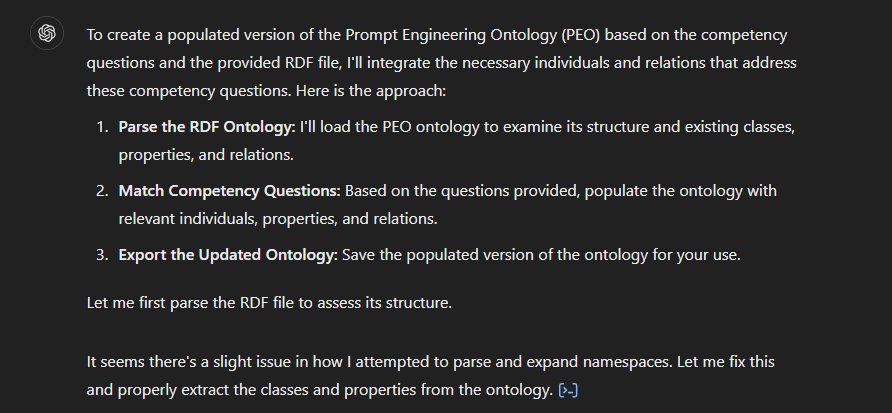
\includegraphics[width=0.9\linewidth]{Figures/fig_35.png}
    \caption{First GPT-4 output in the automatic population}
    \label{fig:enter-label}
\end{figure}
Then the model analyses the ontology structure encoded in the RDF file, listing simple classes and sample object properties found:
\begin{figure}[H]
    \centering
    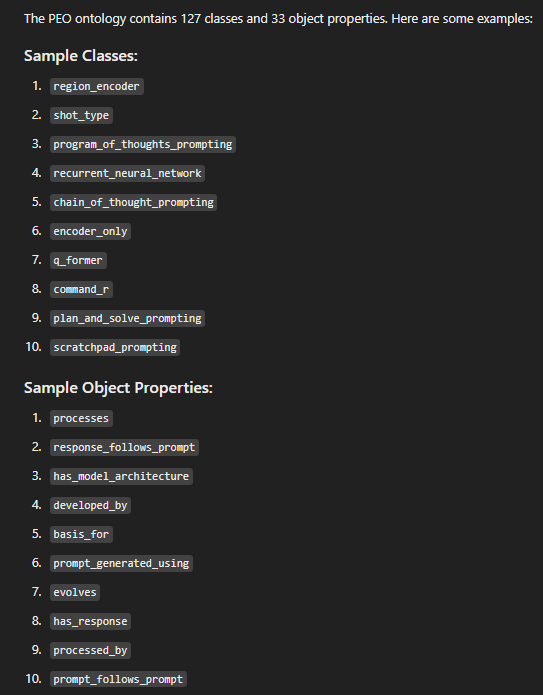
\includegraphics[width=0.85\linewidth]{Figures/fig_36.png}
    \caption{Structure analysis of the ontology}
    \label{fig:enter-label}
\end{figure}
Finally it produces the downloadable RDF file containing the ontology populated by the model:
\begin{figure}[H]
    \centering
    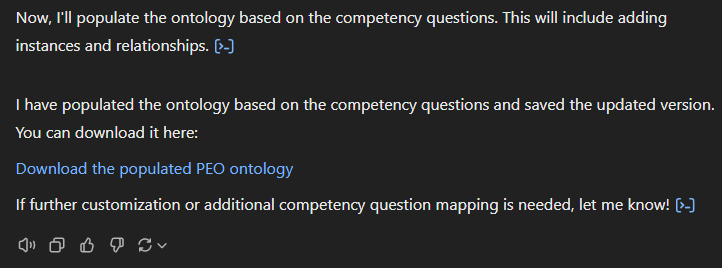
\includegraphics[width=0.9\linewidth]{Figures/fig_37.png}
    \caption{Final LLM output}
    \label{fig:enter-label}
\end{figure}
After downloading the RDF file, I open it using the Protegé editor to see the final result. At a first glance, the obtained result seems rather poor, as four new classes have been created again without considering the classes already present in the ontology:
\begin{itemize}
    \item \textbf{PromptEngineering}
    \item \textbf{Prompt}
    \item \textbf{PromptingTechnique}
    \item \textbf{Task}
\end{itemize}
without considering the hierarchy defined in the ontology as we can see:
\begin{figure}[H]
    \centering
    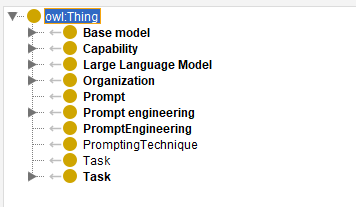
\includegraphics[width=0.9\linewidth]{Figures/fig_38.png}
    \caption{PEO ontology populated automatically}
    \label{fig:enter-label}
\end{figure}
Just two classes have a definition: Prompt and PromptEngineering with no individuals created while the PromptingTechnique class has no defintion and three individuals created:
\begin{itemize}
    \item ChainOfThoughtPrompting
    \item FewShotPrompting
    \item ZeroShotPrompting
\end{itemize}
There is no new instance of chat and all the mechanism defined to link a prompting technique with a chat is completely ignored. No new object properties or data properties have been created by GPT-4o, just an annotation property called \textit{hasDefinition}. Any other useful information is not created, the three entities are not linked with any object property and they do not have any data property. Additional prompts would clearly be needed as input for the large language model to improve the result, which is currently poor and adds no useful information compared to the original, manually populated version of the prompt engineering ontology.

\newpage
\section{Ontology evaluation}
\subsection{Ontology consistency check}
The ontology consistency check consists in running the reasoner in order to check the consistency of declared and inferenced classes and axioms, inferences are made using also SWRL rules described in the encoding section. Running the reasoner ensures also the declaration of disjointness among disjoint classes. I run the HermiT reasoner on both version of the PEO ontology: the version populated manually and the updated version made by GPT-4.\\
On the original version of the PEO ontology, the reasoner does not give any inconsistency and all the axioms are inferred correctly as we cans see below:
\begin{figure}[H]
    \centering
    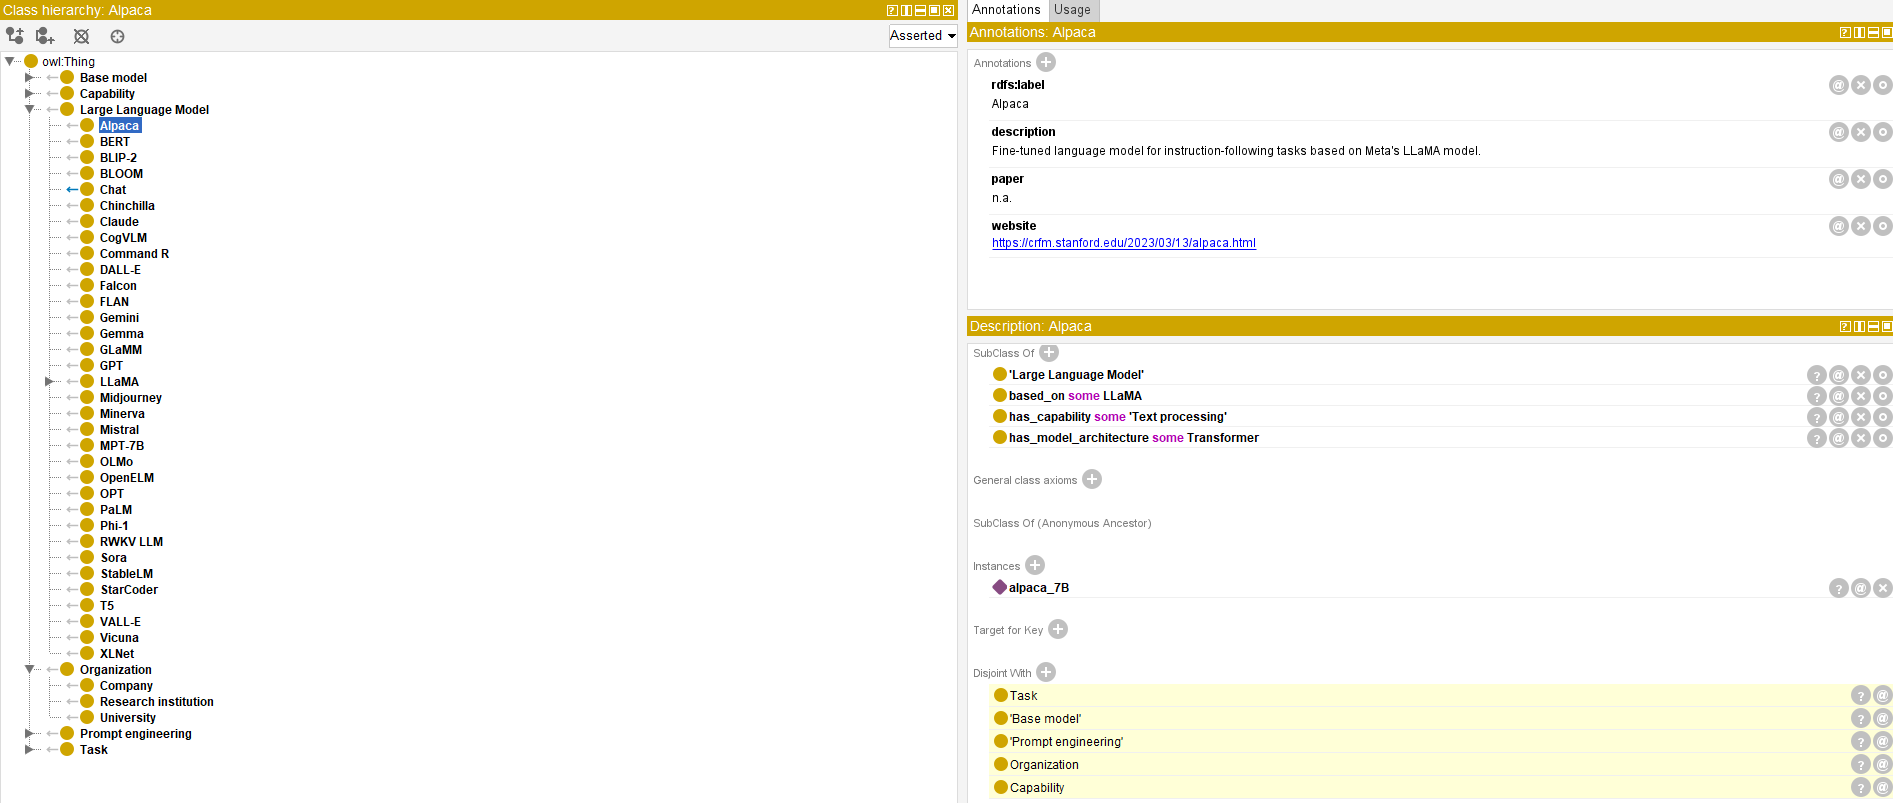
\includegraphics[width=0.9\linewidth]{Figures/fig_39.png}
    \caption{PEO ontology with HermiT reasoner}
    \label{fig:enter-label}
\end{figure}
The reasoner infers correctly that the class "Alpaca" is disjoint with the classes "Task", "Base model", "Prompt engineering", "Organization" and "Capability" because the superclass "Large language model" is declared disjoint with that list of classes. The ten SWRL rules declared work properly and inference the correct object properties for individuals:
\begin{figure}[H]
    \centering
    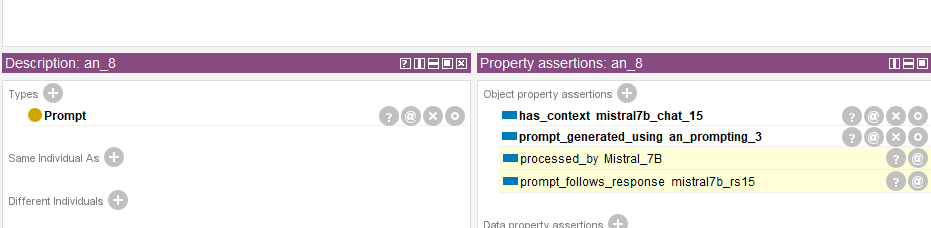
\includegraphics[width=0.9\linewidth]{Figures/fig_40.png}
    \caption{Inference on prompt individual}
    \label{fig:enter-label}
\end{figure}
The consistency check of the other version of the PEO ontology, the one populated using GPT-4 has given the exact results, this because as said in the previous section no additional significant information has been added to the ontology. The inserted classes have no link with other classes so there are no other new inferences.

\subsection{OntoMetrics}
The calculation of metrics is done using OntoMetrics: a web-based tool developed by the University of Rostock that validates and provides statistical analyses of ontologies.\cite{lantow2016ontometrics}
Given the ontology in form of RDF file or code, it calculates automatically:
\begin{itemize}
    \item Base metrics: these include simple counts of ontology elements such as classes, axioms, and objects, providing a quantitative overview of the ontology's components.

    \item Schema Metrics: these metrics evaluate the structure of the ontology's schema, considering aspects like attribute richness and inheritance richness.

    \item Knowledge base Metrics: these assess the ontology's knowledge base, focusing on the population of instances within the ontology.

    \item Class Metrics: these metrics analyse individual classes within the ontology, examining factors such as class connectivity and fullness.

    \item Graph Metrics: these evaluate the ontology's taxonomy as a graph, measuring properties like depth and breadth.
\end{itemize}
For PEO ontology, I will calculate base metrics, schema metrics and graph metrics.
\begin{figure}[H]
    \centering
    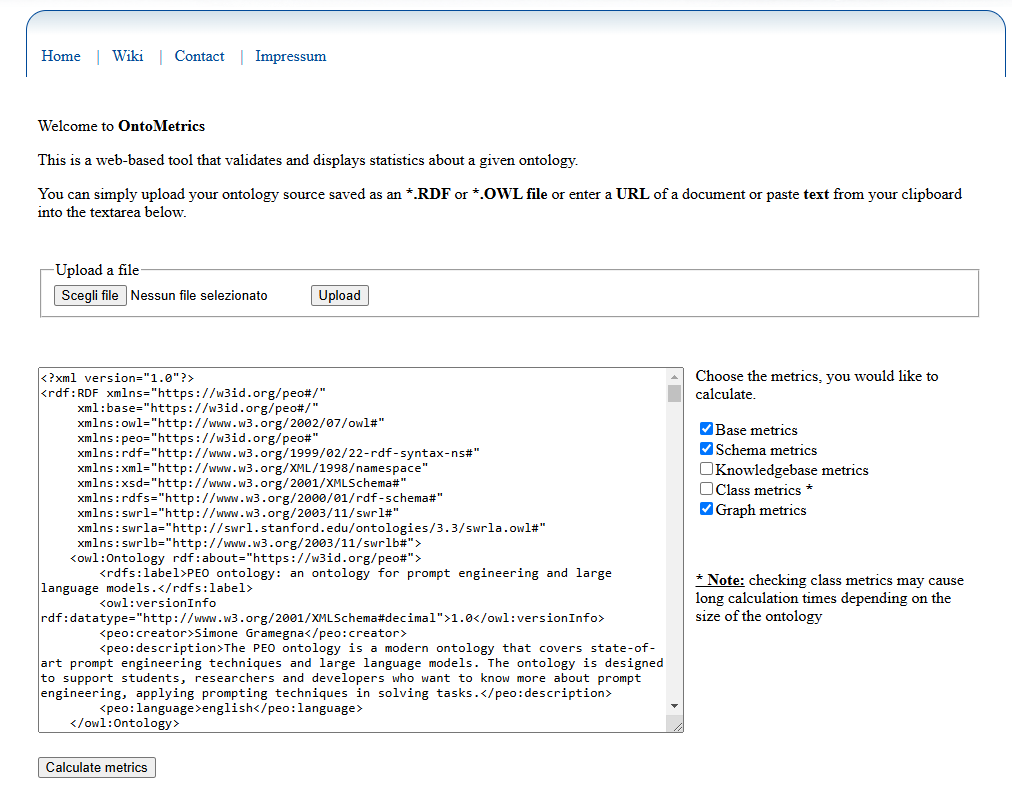
\includegraphics[width=0.9\linewidth]{Figures/fig_41.png}
    \caption{OntoMetrics interface}
    \label{fig:enter-label}
\end{figure}

Values computed for \textbf{base metrics} are:

\begin{table}[H]
    \centering
    \begin{tabular}{|>{\raggedright\arraybackslash}p{8cm}|>{\raggedright\arraybackslash}p{4cm}|}
        \hline
        \textbf{Property} & \textbf{Value} \\ \hline
        Axioms & 2684 \\ \hline
        Logical axioms count & 1695 \\ \hline
        Class count & 126 \\ \hline
        Total classes count & 126 \\ \hline
        Object property count & 34 \\ \hline
        Total object properties count & 34 \\ \hline
        Data property count & 13 \\ \hline
        Total data properties count & 13 \\ \hline
        Properties count & 47 \\ \hline
        Individual count & 352 \\ \hline
        Total individuals count & 352 \\ \hline
        DL expressivity & SRIF(D) \\ \hline
    \end{tabular}
    \caption{PEO ontology base metrics statistics}
    \label{tab:ontology-stats}
\end{table}
This table provides a high-level overview of the ontology’s structure and complexity. With 2684 axioms, the ontology is rich in detail and represents a substantial body of knowledge. Among these, 1695 logical axioms indicate a strong focus on enabling inference and reasoning. The 126 classes show that the ontology has a robust framework for organizing concepts, while 34 object properties and 13 data properties highlight the ontology’s emphasis on relationships over attribute-driven modeling. The inclusion of 352 individuals suggests that the ontology is well-populated, demonstrating practical applicability. The expressivity of SRIF(D) indicates that the ontology supports features like inverse roles and data ranges, balancing computational efficiency with expressive capability. This ontology is comprehensive but may require optimization to handle its inherent complexity effectively.

\begin{table}[H]
    \centering
    \begin{tabular}{|>{\raggedright\arraybackslash}p{8cm}|>{\raggedright\arraybackslash}p{4cm}|}
        \hline
        \textbf{Class Axiom Type} & \textbf{Count} \\ \hline
        SubClassOf axioms count & 199 \\ \hline
        Equivalent classes axioms count & 1 \\ \hline
        Disjoint classes axioms count & 3 \\ \hline
        GCICount & 0 \\ \hline
        HiddenGCICount & 0 \\ \hline
    \end{tabular}
    \caption{PEO ontology Class Axioms statistics}
    \label{tab:class-axioms}
\end{table}

This table details how classes are defined and interrelated within the ontology. The 199 SubClassOf axioms form a strong hierarchical backbone, enabling inheritance of properties and constraints. However, the limited use of equivalent classes (1) and disjoint classes (3) suggests that the ontology may not fully capture nuanced relationships or enforce strict separations between certain concepts. The absence of GCIs (Global Cardinality Restrictions) and Hidden GCIs could indicate missed opportunities to model constraints and relationships that extend across the ontology as a whole. While the current setup simplifies reasoning, incorporating more advanced axioms could enhance the ontology's semantic richness and utility.


\begin{table}[H]
    \centering
    \begin{tabular}{|>{\raggedright\arraybackslash}p{8cm}|>{\raggedright\arraybackslash}p{4cm}|}
        \hline
        \textbf{Object Property Axiom Type} & \textbf{Count} \\ \hline
        SubObjectPropertyOf axioms count & 33 \\ \hline
        Equivalent object properties axioms count & 0 \\ \hline
        Inverse object properties axioms count & 16 \\ \hline
        Disjoint object properties axioms count & 0 \\ \hline
        Functional object properties axioms count & 0 \\ \hline
        Inverse functional object properties axioms count & 0 \\ \hline
        Transitive object property axioms count & 2 \\ \hline
        Symmetric object property axioms count & 0 \\ \hline
        Asymmetric object property axioms count & 0 \\ \hline
        Reflexive object property axioms count & 0 \\ \hline
        Irreflexive object property axioms count & 1 \\ \hline
        Object property domain axioms count & 33 \\ \hline
        Object property range axioms count & 33 \\ \hline
        SubPropertyChainOf axioms count & 0 \\ \hline
    \end{tabular}
    \caption{PEO ontology Object Property Axioms Statistics}
    \label{tab:object-property-axioms}
\end{table}
Object properties are the backbone of the ontology's relational structure. With 33 SubObjectPropertyOf axioms, the ontology defines a clear hierarchy of relationships, which helps maintain organization and reasoning efficiency. The 16 inverse object properties highlight a good use of bidirectional relationships, enhancing navigability within the graph. However, the lack of functional, inverse functional, symmetric, or asymmetric properties may limit the ontology’s ability to capture specific constraints, such as unique or one-to-one relationships. The two transitive properties and one irreflexive property add some complexity but are underused. Domains and ranges are well-defined for all object properties, which is a strong point, as it ensures consistency and logical soundness in property usage.

\begin{table}[H]
    \centering
    \begin{tabular}{|>{\raggedright\arraybackslash}p{8cm}|>{\raggedright\arraybackslash}p{4cm}|}
        \hline
        \textbf{Data Property Axiom Type} & \textbf{Count} \\ \hline
        SubDataPropertyOf axioms count & 12 \\ \hline
        Equivalent data properties axioms count & 0 \\ \hline
        Disjoint data properties axioms count & 0 \\ \hline
        Functional data property axioms count & 7 \\ \hline
        Data property domain axioms count & 11 \\ \hline
        Data property range axioms count & 12 \\ \hline
    \end{tabular}
    \caption{PEO ontology Data Property Axioms Statistics}
    \label{tab:data-property-axioms}
\end{table}

Data properties focus on attributes of individuals. The 12 SubDataPropertyOf axioms indicate some level of organization, but the absence of equivalent or disjoint data properties suggests limited semantic relationships among these properties. Seven functional data properties point to a partial emphasis on ensuring that certain attributes have unique values (e.g., “hasID”), but this aspect could be expanded. Domains and ranges are defined for most properties, which improves clarity and reasoning, but the relatively low overall count of data property axioms might limit the ontology's ability to model detailed attributes of classes or individuals.

\begin{table}[H]
    \centering
    \begin{tabular}{|>{\raggedright\arraybackslash}p{8cm}|>{\raggedright\arraybackslash}p{4cm}|}
        \hline
        \textbf{Individual Axiom Type} & \textbf{Count} \\ \hline
        Class assertion axioms count & 352 \\ \hline
        Object property assertion axioms count & 390 \\ \hline
        Data property assertion axioms count & 580 \\ \hline
        Negative object property assertion axioms count & 0 \\ \hline
        Negative data property assertion axioms count & 0 \\ \hline
        Same individuals axioms count & 0 \\ \hline
        Different individuals axioms count & 0 \\ \hline
    \end{tabular}
    \caption{PEO ontology Individual Axioms Statistics}
    \label{tab:individual-axioms}
\end{table}

This table reflects how individuals are represented and connected within the ontology. The 352 class assertions and 390 object property assertions indicate that the ontology’s individuals are well-categorized and interlinked. The 580 data property assertions further show that these individuals have descriptive attributes. However, the absence of negative assertions (both object and data properties) and no axioms for declaring individuals as equivalent or distinct may limit the ontology's ability to handle complex scenarios, such as resolving conflicts or managing redundancy.

\begin{table}[H]
    \centering
    \begin{tabular}{|>{\raggedright\arraybackslash}p{8cm}|>{\raggedright\arraybackslash}p{4cm}|}
        \hline
        \textbf{Annotation Axiom Type} & \textbf{Count} \\ \hline
        Annotation axioms count & 5 \\ \hline
        Annotation assertion axioms count & 459 \\ \hline
        Annotation property domain axioms count & 0 \\ \hline
        Annotation property range axioms count & 0 \\ \hline
    \end{tabular}
    \caption{PEO ontology Annotation Axioms Statistics}
    \label{tab:annotation-axioms}
\end{table}
Annotations are crucial for documentation and understanding. With 459 annotation assertions, the ontology appears well-documented, providing metadata that can improve usability and comprehension. However, the absence of domain and range axioms for annotation properties suggests that these annotations are not constrained formally, which could lead to inconsistencies or reduced clarity in large-scale applications. Better structuring of annotation properties could enhance the ontology’s maintainability.\\
The \textbf{Schema metrics} computed for PEO ontology are: 

\begin{table}[H]
    \centering
    \begin{tabular}{|>{\raggedright\arraybackslash}p{8cm}|>{\raggedright\arraybackslash}p{4cm}|}
        \hline
        \textbf{Metric} & \textbf{Value} \\ \hline
        Attribute richness & 0.103175 \\ \hline
        Inheritance richness & 1.579365 \\ \hline
        Relationship richness & 0.160338 \\ \hline
        Attribute class ratio & 0.0 \\ \hline
        Equivalence ratio & 0.007937 \\ \hline
        Axiom/class ratio & 21.301587 \\ \hline
        Inverse relations ratio & 0.390244 \\ \hline
        Class/relation ratio & 0.531646 \\ \hline
    \end{tabular}
    \caption{PEO ontology Schema Metrics}
    \label{tab:ontology-metrics}
\end{table}
This table evaluates the structural aspects of the ontology. The attribute richness (0.103175) indicates that relatively few classes have associated attributes, which could limit the detail available for each class. The inheritance richness (1.579365) shows that most classes are part of meaningful hierarchies, a positive sign of structure. However, the relationship richness (0.160338) is relatively low, suggesting that the ontology focuses more on defining concepts than on interconnecting them. The axiom-to-class ratio (21.301587) highlights a dense ontology, meaning each class has substantial associated information, which can be both a strength and a source of complexity. Finally, the inverse relations ratio (0.390244) indicates a good but incomplete use of inverse properties to enhance navigability.\\
The \textbf{Graph metrics} for PEO ontology are:
\begin{table}[H]
    \centering
    \begin{tabular}{|>{\raggedright\arraybackslash}p{8cm}|>{\raggedright\arraybackslash}p{4cm}|}
        \hline
        \textbf{Metric} & \textbf{Value} \\ \hline
        Absolute root cardinality & 7 \\ \hline
        Absolute leaf cardinality & 109 \\ \hline
        Absolute sibling cardinality & 126 \\ \hline
        Absolute depth & 318 \\ \hline
        Average depth & 2.52381 \\ \hline
        Maximal depth & 4 \\ \hline
        Absolute breadth & 126 \\ \hline
        Average breadth & 7.0 \\ \hline
        Maximal breadth & 33 \\ \hline
        Ratio of leaf fan-outness & 0.865079 \\ \hline
        Ratio of sibling fan-outness & 1.0 \\ \hline
        Tangledness & 0.269841 \\ \hline
        Total number of paths & 126 \\ \hline
        Average number of paths & 31.5 \\ \hline
    \end{tabular}
    \caption{PEO ontology Graph Metrics}
    \label{tab:cardinality-depth-metrics}
\end{table}
Graph metrics provide insights into the topology of the ontology. The absolute root cardinality (7) and absolute leaf cardinality (109) indicate a moderately deep hierarchy with good granularity at the leaf level. The maximal depth (4) and average depth (2.52381) suggest a shallow graph, which can make the ontology easier to understand but may oversimplify complex domains. The tangledness (0.269841) is moderate, indicating a graph structure that is connected but not overly complex. The high sibling fan-out ratio (1.0) shows that sibling classes are evenly distributed, while the ratio of leaf fan-outness (0.865079) implies a balanced spread of subclasses from intermediate nodes.\\
Despite there being no significant differences between the original version of the PEO ontology and the version populated using GPT-4, I proceed to calculate metrics.\\
Values computed for base metrics are:
\begin{table}[H]
    \centering
    \begin{tabular}{|>{\raggedright\arraybackslash}p{8cm}|>{\raggedright\arraybackslash}p{4cm}|}
        \hline
        \textbf{Property} & \textbf{Value} \\ \hline
        Axioms & 2705 \\ \hline
        Logical axioms count & 1710 \\ \hline
        Class count & 128 \\ \hline
        Total classes count & 128 \\ \hline
        Object property count & 34 \\ \hline
        Total object properties count & 34 \\ \hline
        Data property count & 13 \\ \hline
        Total data properties count & 13 \\ \hline
        Properties count & 47 \\ \hline
        Individual count & 359 \\ \hline
        Total individuals count & 359 \\ \hline
        DL expressivity & SRIF(D) \\ \hline
    \end{tabular}
    \caption{PEO ontology updated base metrics statistics}
    \label{tab:ontology-stats-updated}
\end{table}

\begin{table}[H]
    \centering
    \begin{tabular}{|>{\raggedright\arraybackslash}p{8cm}|>{\raggedright\arraybackslash}p{4cm}|}
        \hline
        \textbf{Class Axiom Type} & \textbf{Count} \\ \hline
        SubClassOf axioms count & 197 \\ \hline
        Equivalent classes axioms count & 1 \\ \hline
        Disjoint classes axioms count & 3 \\ \hline
        GCICount & 0 \\ \hline
        HiddenGCICount & 0 \\ \hline
    \end{tabular}
    \caption{PEO ontology updated Class Axioms Statistics}
    \label{tab:class-axioms-updated}
\end{table}

\begin{table}[H]
    \centering
    \begin{tabular}{|>{\raggedright\arraybackslash}p{8cm}|>{\raggedright\arraybackslash}p{4cm}|}
        \hline
        \textbf{Object Property Axiom Type} & \textbf{Count} \\ \hline
        SubObjectPropertyOf axioms count & 33 \\ \hline
        Equivalent object properties axioms count & 0 \\ \hline
        Inverse object properties axioms count & 16 \\ \hline
        Disjoint object properties axioms count & 0 \\ \hline
        Functional object properties axioms count & 0 \\ \hline
        Inverse functional object properties axioms count & 0 \\ \hline
        Transitive object property axioms count & 8 \\ \hline
        Symmetric object property axioms count & 1 \\ \hline
        Asymmetric object property axioms count & 0 \\ \hline
        Reflexive object property axioms count & 0 \\ \hline
        Irreflexive object property axioms count & 1 \\ \hline
        Object property domain axioms count & 33 \\ \hline
        Object property range axioms count & 33 \\ \hline
        SubPropertyChainOf axioms count & 0 \\ \hline
    \end{tabular}
    \caption{PEO ontology updated Object Property Axioms Statistics}
    \label{tab:object-property-axioms-updated}
\end{table}

\begin{table}[H]
    \centering
    \begin{tabular}{|>{\raggedright\arraybackslash}p{8cm}|>{\raggedright\arraybackslash}p{4cm}|}
        \hline
        \textbf{Data Property Axiom Type} & \textbf{Count} \\ \hline
        SubDataPropertyOf axioms count & 12 \\ \hline
        Equivalent data properties axioms count & 0 \\ \hline
        Disjoint data properties axioms count & 0 \\ \hline
        Functional data property axioms count & 7 \\ \hline
        Data property domain axioms count & 12 \\ \hline
        Data property range axioms count & 12 \\ \hline
    \end{tabular}
    \caption{PEO ontology updated Data Property Axioms Statistics}
    \label{tab:data-property-axioms-updated}
\end{table}

\begin{table}[H]
    \centering
    \begin{tabular}{|>{\raggedright\arraybackslash}p{8cm}|>{\raggedright\arraybackslash}p{4cm}|}
        \hline
        \textbf{Individual Axiom Type} & \textbf{Count} \\ \hline
        Class assertion axioms count & 358 \\ \hline
        Object property assertion axioms count & 393 \\ \hline
        Data property assertion axioms count & 580 \\ \hline
        Negative object property assertion axioms count & 0 \\ \hline
        Negative data property assertion axioms count & 0 \\ \hline
        Same individuals axioms count & 0 \\ \hline
        Different individuals axioms count & 0 \\ \hline
    \end{tabular}
    \caption{PEO ontology updated Individual Axioms Statistics}
    \label{tab:individual-axioms-updated}
\end{table}

\begin{table}[H]
    \centering
    \begin{tabular}{|>{\raggedright\arraybackslash}p{8cm}|>{\raggedright\arraybackslash}p{4cm}|}
        \hline
        \textbf{Annotation Axiom Type} & \textbf{Count} \\ \hline
        Annotation axioms count & 5 \\ \hline
        Annotation assertion axioms count & 456 \\ \hline
        Annotation property domain axioms count & 0 \\ \hline
        Annotation property range axioms count & 0 \\ \hline
    \end{tabular}
    \caption{PEO ontology updated Annotation Axioms Statistics}
    \label{tab:annotation-axioms-updated}
\end{table}

The schema metrics for the update version of PEO ontology are:
\begin{table}[H]
    \centering
    \begin{tabular}{|>{\raggedright\arraybackslash}p{8cm}|>{\raggedright\arraybackslash}p{4cm}|}
        \hline
        \textbf{Metric} & \textbf{Value} \\ \hline
        Attribute richness & 0.101563 \\ \hline
        Inheritance richness & 1.539063 \\ \hline
        Relationship richness & 0.161702 \\ \hline
        Attribute class ratio & 0.0 \\ \hline
        Equivalence ratio & 0.007813 \\ \hline
        Axiom/class ratio & 21.132813 \\ \hline
        Inverse relations ratio & 0.390244 \\ \hline
        Class/relation ratio & 0.544681 \\ \hline
    \end{tabular}
    \caption{PEO ontology Schema Metrics}
    \label{tab:ontology-metrics-updated}
\end{table}

The graph metrics for updated version of PEO ontology are:

\begin{table}[H]
    \centering
    \begin{tabular}{|>{\raggedright\arraybackslash}p{8cm}|>{\raggedright\arraybackslash}p{4cm}|}
        \hline
        \textbf{Metric} & \textbf{Value} \\ \hline
        Absolute root cardinality & 11 \\ \hline
        Absolute leaf cardinality & 111 \\ \hline
        Absolute sibling cardinality & 128 \\ \hline
        Absolute depth & 316 \\ \hline
        Average depth & 2.46875 \\ \hline
        Maximal depth & 4 \\ \hline
        Absolute breadth & 128 \\ \hline
        Average breadth & 7.111111 \\ \hline
        Maximal breadth & 33 \\ \hline
        Ratio of leaf fan-outness & 0.867188 \\ \hline
        Ratio of sibling fan-outness & 1.0 \\ \hline
        Tangledness & 0.265625 \\ \hline
        Total number of paths & 128 \\ \hline
        Average number of paths & 32.0 \\ \hline
    \end{tabular}
    \caption{PEO ontology updated Graph Metrics}
    \label{tab:cardinality-depth-metrics-updated}
\end{table}
The new values calculated by OntoMetrics on the updated version of the ontology do not differ significantly from the previously calculated values, as the large language model GPT-4 has only added four new classes and three new instances. All results for PEO ontology and its second version are on \href{https://github.com/simonegramegna/peo/tree/main/evaluation}{Github}.

\newpage
\subsection{OOPS! validation}
The methods discussed so far are widely used in ontology evaluation; however, they are not capable of capturing modelling errors in greater detail. These errors can compromise not only the quality and usability of the ontology but also lead to potential inconsistencies. Therefore, it is necessary to adopt a different approach from those previously examined, OntoMetrics and the HermiT reasoner because they have the following issues:
\begin{itemize}
    \item OntoMetrics: it provides a quantitative measure of ontology's structural characteristics without analysing qualitative aspects, so it is not able to detect semantic and usability issues in the ontology.

    \item HermiT reasoner (reasoners in general): reasoners are designed to check the logical consistency of an ontology and perform inferencing identifying inconsistencies in axioms. But reasoners are not able to detect errors outside logical inconsistencies, such as missing domain or range definitions and they cannot check best-practice violation and usability issues.
\end{itemize}
These limitations highlight the need for a tool that can go beyond structural and logical evaluation, addressing both semantic and usability dimensions of ontology quality. \textbf{OOPS!} (Ontology Pitfall Scanner) is an online tool for ontology evaluation \cite{poveda2014oops} that automates the evaluation process without requiring any effort by the developer. 
\begin{figure}[H]
    \centering
    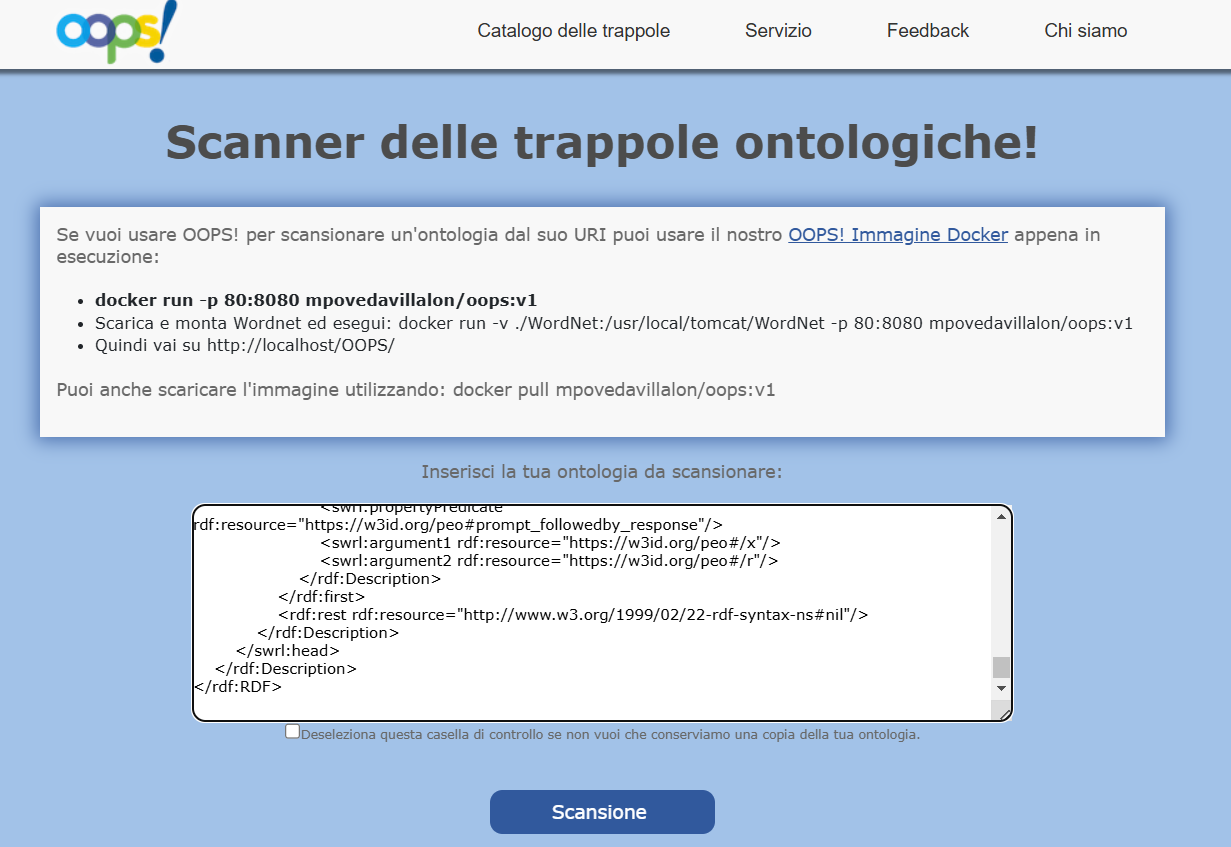
\includegraphics[width=0.9\linewidth]{Figures/fig_42.png}
    \caption{OOPS! web interface}
    \label{fig:enter-label}
\end{figure}
Given the input ontology, OOPS is able to detect 40 different pitfall that are classified into three categories: critical, important and minor by parsing the RDF code and generating a complete response using the OOPS! scanner. Pitfalls in the scanner include:
\begin{itemize}
    \item Structural pitfalls: these involve issues related to the ontology's formal structure and syntax like cycles in hierarchy and unconnected ontology elements.

    \item Functional pitfalls: these involve issues to the intended use and functionality of the ontology like missing domain or incorrectly defined inverse relationships.

    \item Usability and Profiling Pitfalls: these involve issues  affecting the ontology's clarity, maintainability, and human-readability like missing annotations, inconsistent naming and ambiguous terms.
\end{itemize}
I will use OOPS! scanner on both versions of the PEO ontology detecting and explaining found pitfalls. 
For the first version of PEO ontology there are just three pitfalls:
\begin{figure}[H]
    \centering
    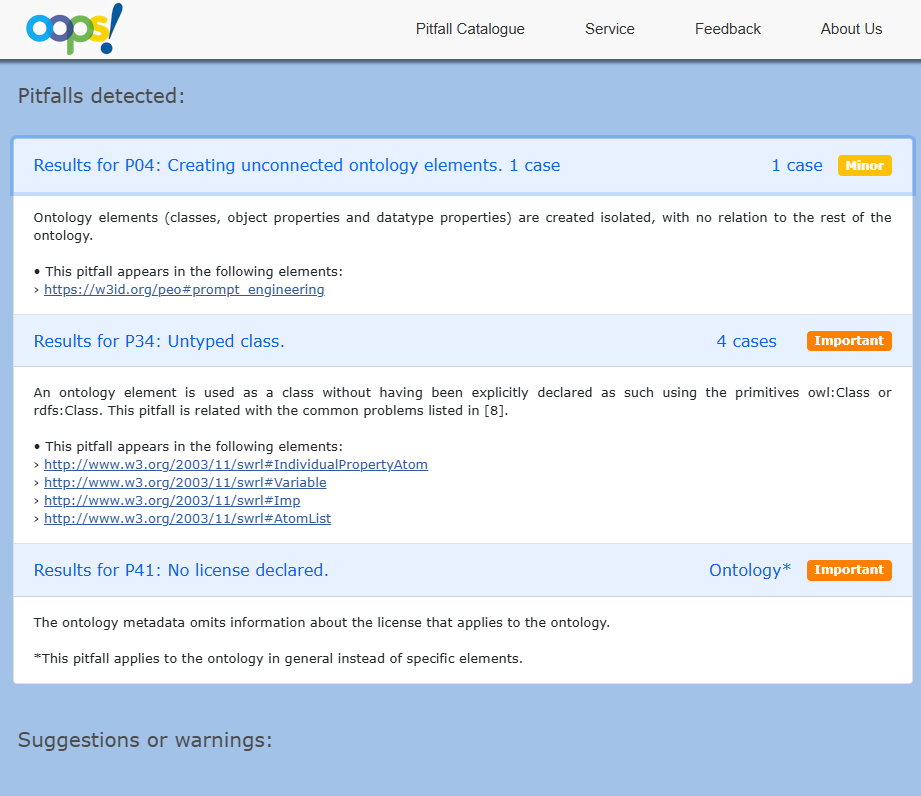
\includegraphics[width=0.9\linewidth]{Figures/fig_43.png}
    \caption{Detected pitfalls PEO ontology}
    \label{fig:enter-label}
\end{figure}
The explanation of detected pitfall is:
\begin{itemize}
    \item \textbf{P04 (Creating unconnected ontology elements):} this pitfall involves ontology elements (classes, object properties and datatype properties) are created isolated, with no relation to the rest of the ontology. In the case of PEO ontology, the \textit{prompt\_engineering} class has no relation: this because the prompt engineering class is intended as a theoretical concept with no relations with other classes.

    \item \textbf{P34 (Untyped class):} this pitfalls involves all ontology elements that are used as a class without having explicitly declared. This pitfall involves four elements in PEO ontology: \\ \textit{http://www.w3.org/2003/11/swrl\#IndividualPropertyAtom},\\ \textit{http://www.w3.org/2003/11/swrl\#Variable},\\ \textit{http://www.w3.org/2003/11/swrl\#Imp} and \\\textit{http://www.w3.org/2003/11/swrl\#AtomList}.
    This pitfall depends in the declaration of SWRL rules using the Protegé editor and it does not depend on the developer.

    \item \textbf{P41 (No license declared):} there is no license in the ontology metadata. The license of PEO ontology is specified in the Github repository.
    
\end{itemize}
Overall, the report is satisfactory, as no critical pitfalls have been identified, nor any issues found in the main classes or object properties of the ontology. The complete report is available \href{https://github.com/simonegramegna/peo/blob/main/evaluation/oops_report_peo.xml}{here}. After detecting pitfalls in the original version of the PEO ontology, I also examined the populated version generated using GPT-4 nonetheless, no significant differences were observed between the two versions. Compared to the three pitfalls identified in the previous version, OOPS detects five pitfalls:
\begin{figure}[H]
    \centering
    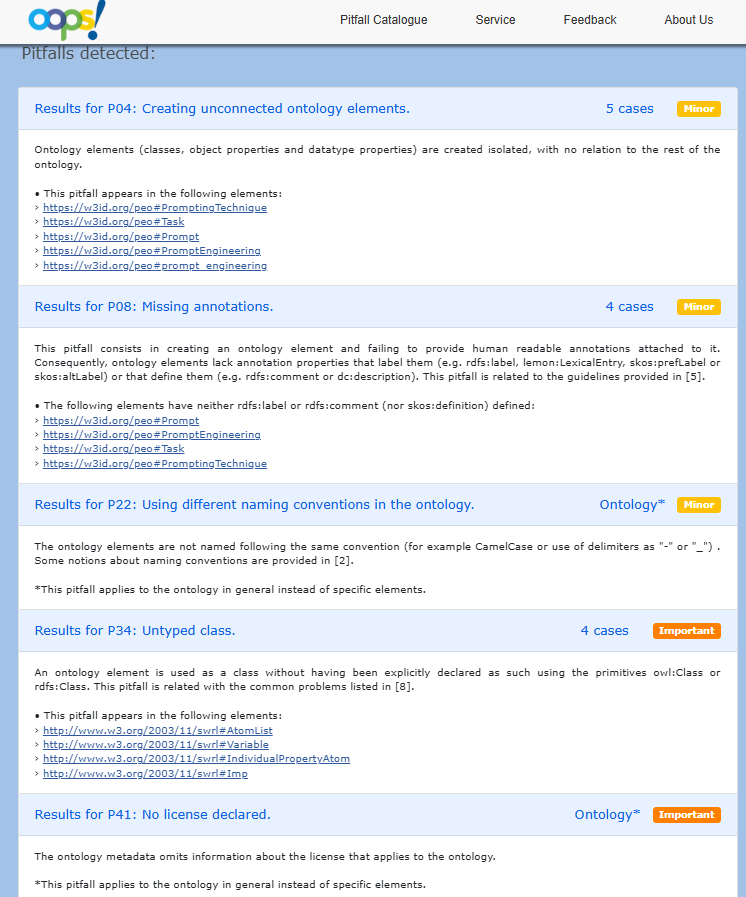
\includegraphics[width=0.75\linewidth]{Figures/fig_44.png}
    \caption{Detected pitfalls second version PEO ontology}
    \label{fig:enter-label}
\end{figure}


\begin{itemize}
    \item \textbf{P04 (Creating unconnected ontology elements):} this pitfall, as said before, involves unconnected ontology elements. This time the pitfall involves not only the \textit{prompt\_engineering} class but also the new classes created by GPT-4: \textit{Task}, \textit{PromptingTechnique}, \textit{Prompt} and \textit{PromptEngineering}. Those classes have no relations with other classes.

    \item \textbf{P08 (Missing annotations):} this pitfall involves elements that lack annotation properties that label them ( \textit{rdfs:label}) or that define them\\ (\textit{rdfs:comment}). This pitall involves the four classes created by GPT-4 with no comment provided: \textit{Task}, \textit{PromptingTechnique}, \textit{Prompt} and \textit{PromptEngineering}.  

    \item \textbf{P22 (Using different naming conventions in the ontology):} this pitfall involves ontology elements are not named following the same convention (for example CamelCase or use of delimiters as "-" or "\_"). This pitfall is given by the new classes created by GPT-4 that do not follow the naming convention used in the ontology (with the "\_" separator) by creating classes declared in camel case.

    \item \textbf{P34 (Untyped class):} this is the same pitfall detected before.

    \item \textbf{P41 (No license declared):} this is the same pitfall detected before.
\end{itemize}
In general, the detected pitfalls are caused by GPT-4's lack of understanding of the ontology's structure. Additionally, they are not numerous, as the modifications made by the LLM are minimal, the oops report is available \href{https://github.com/simonegramegna/peo/blob/main/evaluation/oops_report_peo_gpt4.xml}{here}.


\subsection{SPARQL queries}
The final step of ontology evaluation is converting competency questions (CQ) defined in the \textit{Ontology requirements specification} section into SPARQL queries in order to compare the expected result to the actual result of each competency question. SPARQL queries are generated manually and ran using Jupyter notebook \cite{jupyter}: an enviroment for running python code and the rdflib python library \cite{rdflib}: a library to access rdf files and run SPARQL queries inside python. The code is available on the \href{https://github.com/simonegramegna/peo/tree/main/evaluation}{Github repository} and the evaluation is mode for both versions of the ontology.\\
First I open the ontology using rdflib:
\begin{figure}[H]
    \centering
    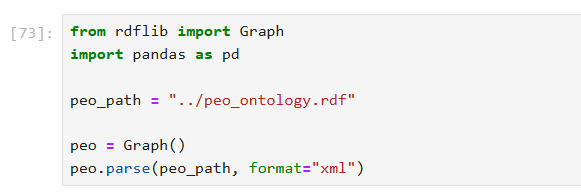
\includegraphics[width=0.9\linewidth]{Figures/fig_45.png}
    \caption{Jupyter notebook SPARQL}
    \label{fig:enter-label}
\end{figure}
The pandas library is used to display query results in data-frames, for query and display I created three support functions: 
\begin{itemize}
    \item \textit{execute\_query:} it takes as input the SPARQL query string and returns a list of results.

    \item \textit{results\_to\_df:} it takes as input as input the list of results ad creates and returns a dataframe with results inside which columns' names are the label names.

    \item \textit{print\_results:} it iterates on the list of results and prints each element.
\end{itemize}
We can see the implementation below:
\begin{figure}[H]
    \centering
    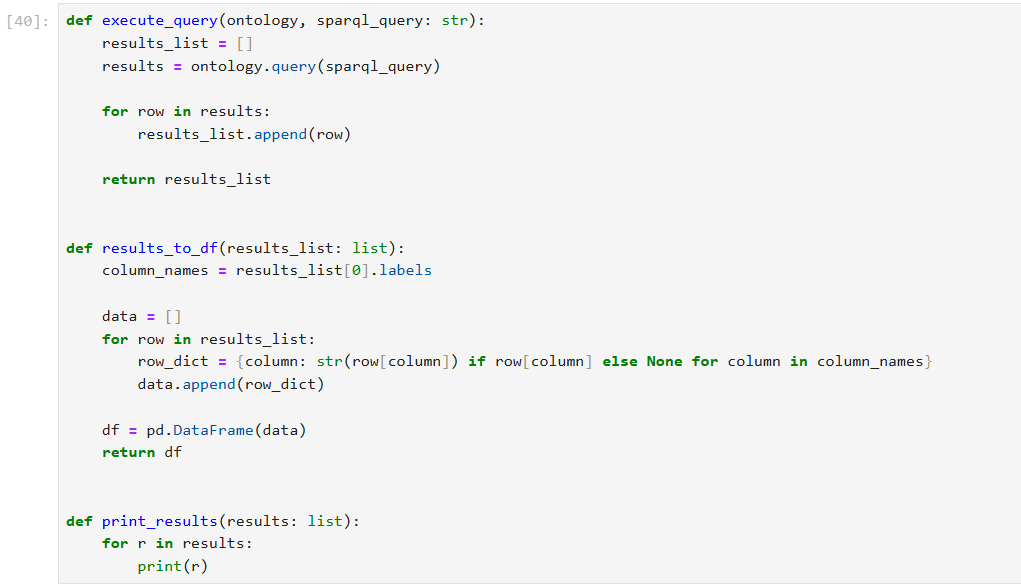
\includegraphics[width=0.9\linewidth]{Figures/fig_46.png}
    \caption{Support python functions}
    \label{fig:enter-label}
\end{figure}
Once this is done, I can translate each of the sixteen competency questions into SPARQL queries to be executed.\\
The first competency question \textbf{CQ1: What is prompt engineering?} is translated into:
\begin{lstlisting}
    SELECT DISTINCT ?property ?value
    WHERE {
        <https://w3id.org/peo#prompt_engineering> ?property ?value .
    }
\end{lstlisting}
Getting the following result:
\begin{figure}[H]
    \centering
    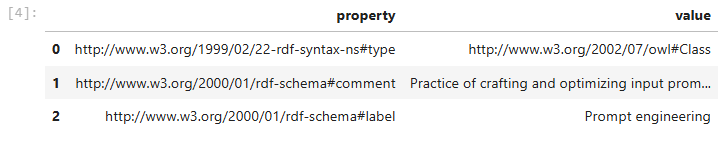
\includegraphics[width=0.9\linewidth]{Figures/fig_47.png}
    \caption{CQ1 SPARQL query results}
    \label{fig:enter-label}
\end{figure}
The output from the query matches the expected result, which is the definition of prompt engineering.\\

The second competency question \textbf{CQ2: What is a prompt?} is translated into:
\begin{lstlisting}
SELECT DISTINCT ?property ?value
WHERE {
    <https://w3id.org/peo#prompt> ?property ?value .
}
\end{lstlisting}
Getting the following results:
\begin{figure}[H]
    \centering
    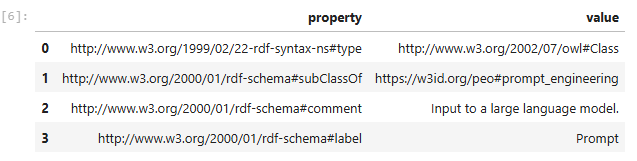
\includegraphics[width=0.9\linewidth]{Figures/fig_48.png}
    \caption{CQ2 SPARQL query results}
    \label{fig:enter-label}
\end{figure}

The output also in this case matches the expected result, which is the definition of prompt.\\

The third competency question \textbf{CQ3: What are prompting techniques?} is translated into:
\begin{lstlisting}
SELECT DISTINCT ?subclass ?label
WHERE {
    ?subclass rdfs:subClassOf <https://w3id.org/peo#prompting_technique> .
    OPTIONAL { ?subclass rdfs:label ?label . }
}
\end{lstlisting}
Getting the following results:
\begin{figure}[H]
    \centering
    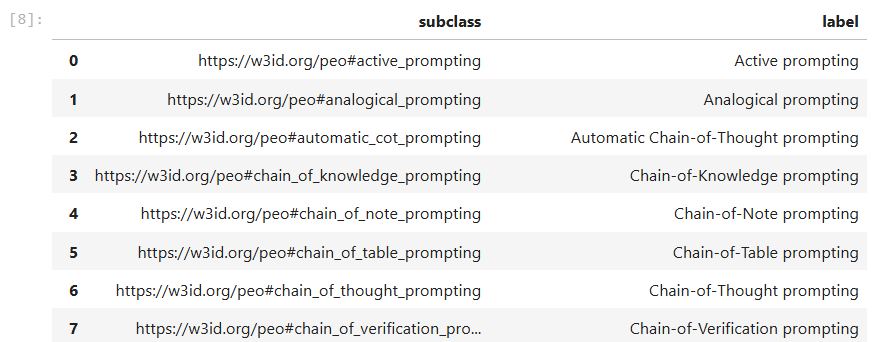
\includegraphics[width=0.9\linewidth]{Figures/fig_49.png}
    \caption{CQ3 SPARQL query results}
    \label{fig:enter-label}
\end{figure}
The complete table contains, as expected, all the prompting techniques in the ontology.\\

The fourth competency question \textbf{CQ4: What are image prompting techniques?} is translated into:
\begin{lstlisting}
SELECT DISTINCT ?subclass ?label
WHERE {
    ?subclass rdfs:subClassOf <https://w3id.org/peo#image_prompting> .
    OPTIONAL { ?subclass rdfs:label ?label . }
}
\end{lstlisting}
Getting the following results:
\begin{figure}[H]
    \centering
    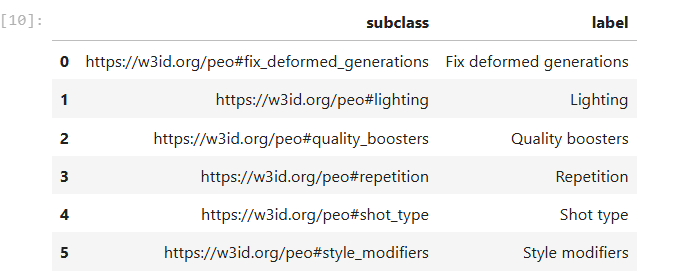
\includegraphics[width=0.9\linewidth]{Figures/fig_50.png}
    \caption{CQ4 SPARQL query results}
    \label{fig:enter-label}
\end{figure}
As expected, we get all the image prompting techniques in the ontology.\\

The fifth competency question \textbf{CQ5: What are code prompting techniques?} is translated into:
\begin{lstlisting}
SELECT DISTINCT ?subclass ?label
WHERE {
    ?subclass rdfs:subClassOf <https://w3id.org/peo#code_prompting> .
    OPTIONAL { ?subclass rdfs:label ?label . }
}  
\end{lstlisting}
Getting the following results:
\begin{figure}[H]
    \centering
    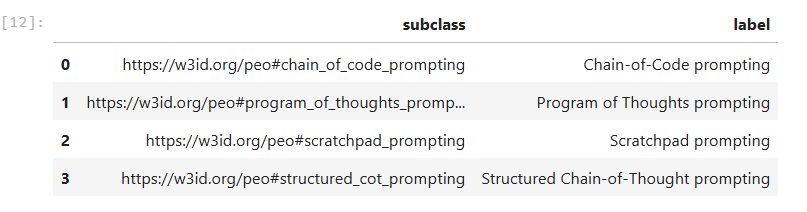
\includegraphics[width=0.9\linewidth]{Figures/fig_51.png}
    \caption{CQ5 SPARQL query results}
    \label{fig:enter-label}
\end{figure}
The table contains, as expected, all the code prompting techniques in the ontology.\\

The sixth competency question \textbf{CQ6: Which task does a prompt solve?} is translated into:
\begin{lstlisting}
SELECT DISTINCT ?prompt ?task ?taskLabel
WHERE {
    ?prompt <https://w3id.org/peo#solves> ?task .
    OPTIONAL { ?task rdfs:label ?taskLabel . }
}
\end{lstlisting}
Getting the following results:
\begin{figure}[H]
    \centering
    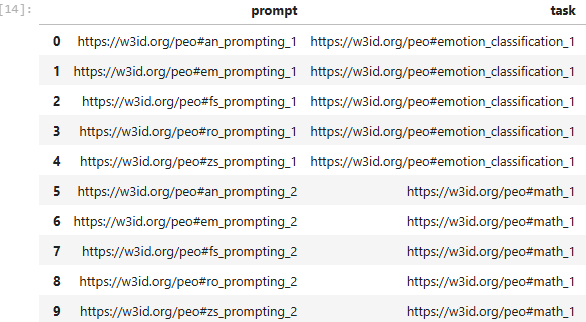
\includegraphics[width=0.9\linewidth]{Figures/fig_52.png}
    \caption{CQ6 SPARQL query results}
    \label{fig:enter-label}
\end{figure}
The table contains, as expected, all the prompts that solve tasks.\\

The seventh competency question \textbf{CQ7: Which prompts are generated using a prompting technique?} is translated into:
\begin{lstlisting}
SELECT DISTINCT ?prompt ?technique ?techniqueLabel
WHERE {
    ?prompt <https://w3id.org/peo#prompt_generated_using> ?technique .
    OPTIONAL { ?technique rdfs:label ?techniqueLabel . }
}
\end{lstlisting}
Getting the following results:
\begin{figure}[H]
    \centering
    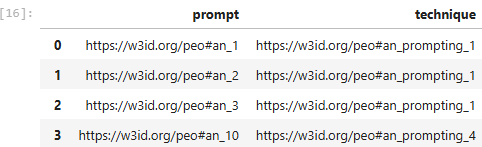
\includegraphics[width=0.9\linewidth]{Figures/fig_53.png}
    \caption{CQ7 SPARQL query results}
    \label{fig:enter-label}
\end{figure}
The complete table, as expected, contains all the prompt instances generated using instances of prompting techniques.\\

The eighth competency question \textbf{CQ8: What are the responses that follow each prompt?} is translated into:
\begin{lstlisting}
SELECT DISTINCT ?prompt ?response
WHERE {
    ?response <https://w3id.org/peo#response_followedby_prompt> ?prompt .
}    
\end{lstlisting}
Getting the following results:
\begin{figure}[H]
    \centering
    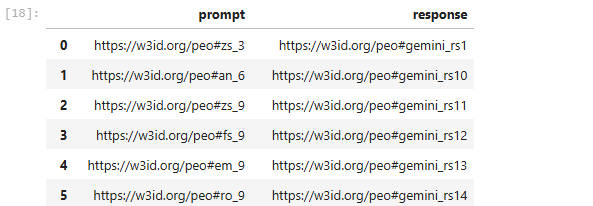
\includegraphics[width=0.9\linewidth]{Figures/fig_54.png}
    \caption{CQ8 SPARQL query results}
    \label{fig:enter-label}
\end{figure}
The complete table contains, as expected, all the responses of all prompt instances.\\

The ninth competency question \textbf{CQ9: What are possible tasks?} is translated into:
\begin{lstlisting}
SELECT DISTINCT ?task ?label
WHERE {
    ?task rdf:type owl:Class .
    ?task rdfs:subClassOf* <https://w3id.org/peo#task> .
    OPTIONAL { ?task rdfs:label ?label . }
}    
\end{lstlisting}
Getting the following results:
\begin{figure}[H]
    \centering
    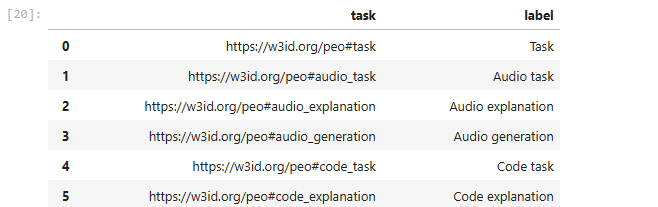
\includegraphics[width=0.9\linewidth]{Figures/fig_55.png}
    \caption{CQ9 SPARQL query results}
    \label{fig:enter-label}
\end{figure}
As expected, in the completed table we get all the possible task represented in the ontology.\\

The tenth competency question \textbf{CQ10: Which tasks are related to the text?} is translated into:
\begin{lstlisting}
SELECT DISTINCT ?task ?label
WHERE {
    ?task rdf:type owl:Class .
    ?task rdfs:subClassOf* <https://w3id.org/peo#text_task> .
    OPTIONAL { ?task rdfs:label ?label . }
}
\end{lstlisting}
Getting the following results:
\begin{figure}[H]
    \centering
    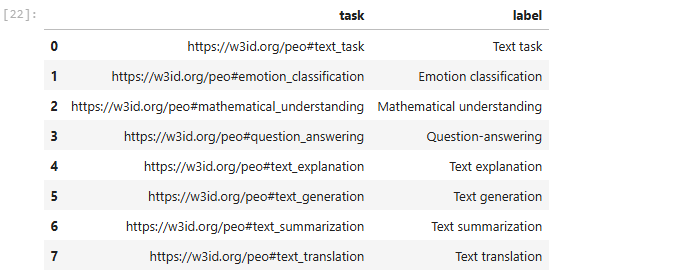
\includegraphics[width=0.9\linewidth]{Figures/fig_56.png}
    \caption{CQ10 SPARQL query results}
    \label{fig:enter-label}
\end{figure}

The resulting table, as expected, contains, all the task related to text.\\

The eleventh competency question \textbf{CQ11: What is a chat?} is translated into:
\begin{lstlisting}
SELECT DISTINCT ?property ?value
WHERE {
    <https://w3id.org/peo#chat> ?property ?value .
}
\end{lstlisting}
Getting the following results:
\begin{figure}[H]
    \centering
    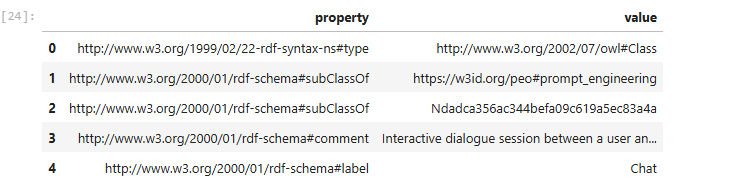
\includegraphics[width=0.9\linewidth]{Figures/fig_57.png}
    \caption{CQ11 SPARQL query results}
    \label{fig:enter-label}
\end{figure}
The result, as expected, is the definition of Chat.\\

The twelfth competency question \textbf{CQ12: What is a large language model?} is translated into:
\begin{lstlisting}
SELECT DISTINCT ?property ?value
WHERE {
    <https://w3id.org/peo#large_language_model> ?property ?value .
}
\end{lstlisting}
Getting the following results:
\begin{figure}[H]
    \centering
    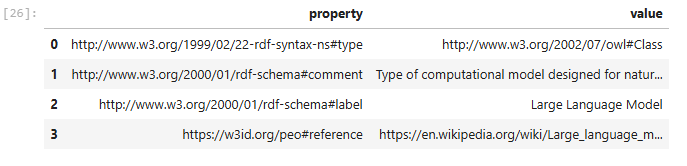
\includegraphics[width=0.9\linewidth]{Figures/fig_58.png}
    \caption{CQ12 SPARQL query results}
    \label{fig:enter-label}
\end{figure}
The result, as expected, is the definition of Large Language Model.\\

The thirteenth competency question \textbf{CQ13: What types of large language models are available?} is translated into:
\begin{lstlisting}
SELECT DISTINCT ?type ?label
WHERE {
    ?type rdfs:subClassOf <https://w3id.org/peo#large_language_model> .
    OPTIONAL { ?type rdfs:label ?label . }
}
\end{lstlisting}
Getting the following results:
\begin{figure}[H]
    \centering
    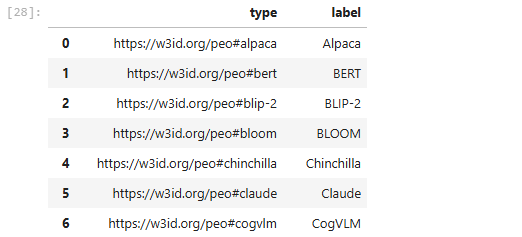
\includegraphics[width=0.9\linewidth]{Figures/fig_59.png}
    \caption{CQ13 SPARQL query results}
    \label{fig:enter-label}
\end{figure}
The resulting complete table, as expected, is the collection of all large language models represented in the ontology.\\

The fourteenth competency question \textbf{CQ14: What are large language models architectures?} is translated into:
\begin{lstlisting}
SELECT DISTINCT ?type ?label
WHERE {
    ?type rdfs:subClassOf <https://w3id.org/peo#base_model> .
    OPTIONAL { ?type rdfs:label ?label . }
}   
\end{lstlisting}
Getting the following results:
\begin{figure}[H]
    \centering
    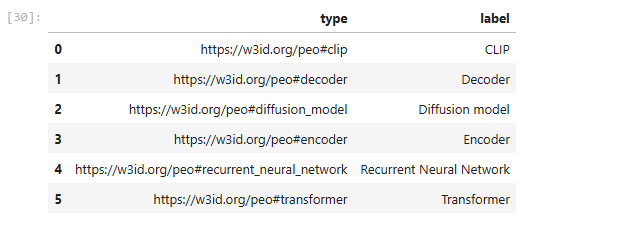
\includegraphics[width=0.9\linewidth]{Figures/fig_60.png}
    \caption{CQ14 SPARQL query results}
    \label{fig:enter-label}
\end{figure}
The result, as expected, is the collection of main large language models architectures.\\

The fifteenth competency question \textbf{CQ15: What are large language models capabilities?} is translated into:
\begin{lstlisting}
SELECT DISTINCT ?type ?label
WHERE {
    ?type rdfs:subClassOf <https://w3id.org/peo#capability> .
    OPTIONAL { ?type rdfs:label ?label . }
}
\end{lstlisting}
Getting the following results:
\begin{figure}[H]
    \centering
    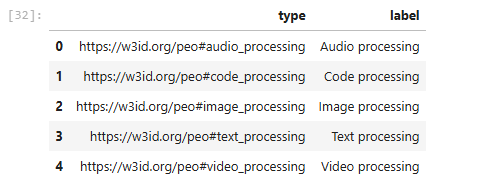
\includegraphics[width=0.8\linewidth]{Figures/fig_61.png}
    \caption{CQ15 SPARQL query results}
    \label{fig:enter-label}
\end{figure}
As expected, the results is the collection of all the capabilities represented in the ontology.\\

The sixteenth and last competency question \textbf{CQ16: What companies develop large language models?} is translated into:
\begin{lstlisting}
SELECT DISTINCT ?company ?label
WHERE {
    ?company rdf:type <https://w3id.org/peo#company> .
    OPTIONAL { ?company rdfs:label ?label . }
}
\end{lstlisting}
Getting the following results:
\begin{figure}[H]
    \centering
    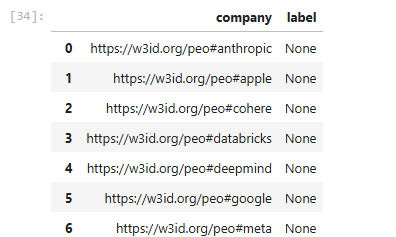
\includegraphics[width=0.8\linewidth]{Figures/fig_62.png}
    \caption{CQ16 SPARQL query results}
    \label{fig:enter-label}
\end{figure}
The result, as expected, is the collection of companies that develop large language models.


\newpage
\section{Ontology publication and maintenance}
The last step after the Ontology implementation in the LOT methodology is the Ontology publication phase, which scope is to provide an online ontology accessible both as human-readable documentation and a machine-readable documentation from its URI. This phase is divided into three sub-activities:
\begin{enumerate}
    \item \textbf{Propose release candidate}
    \item \textbf{Ontology documentation}
    \item \textbf{Online publication}
\end{enumerate}
as we can see in the figure below:
\begin{figure}[H]
    \centering
    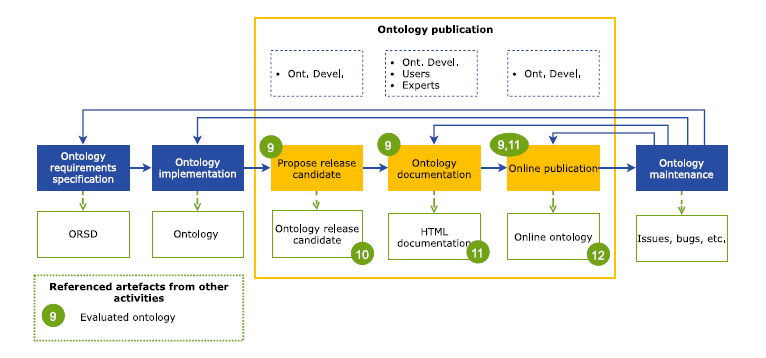
\includegraphics[width=0.9\linewidth]{Figures/fig_25.png}
    \caption{Ontology publication workflow}
    \label{fig:enter-label}
\end{figure}

\subsection{Propose release candidate}
After all the implementation and evaluation, in this step there is the decision about which version of the ontology is going to be published. It is a quite easy choice because, as said in pervious sections, the version populated automatically did not added any useful information from the original version. Moreover it added, according the OOPS! report, more pitfalls (five vs three) so the ontology that is going to be published is the 1.0 version of PEO ontology, populated manually without any llm intervention.
\begin{figure}[H]
    \centering
    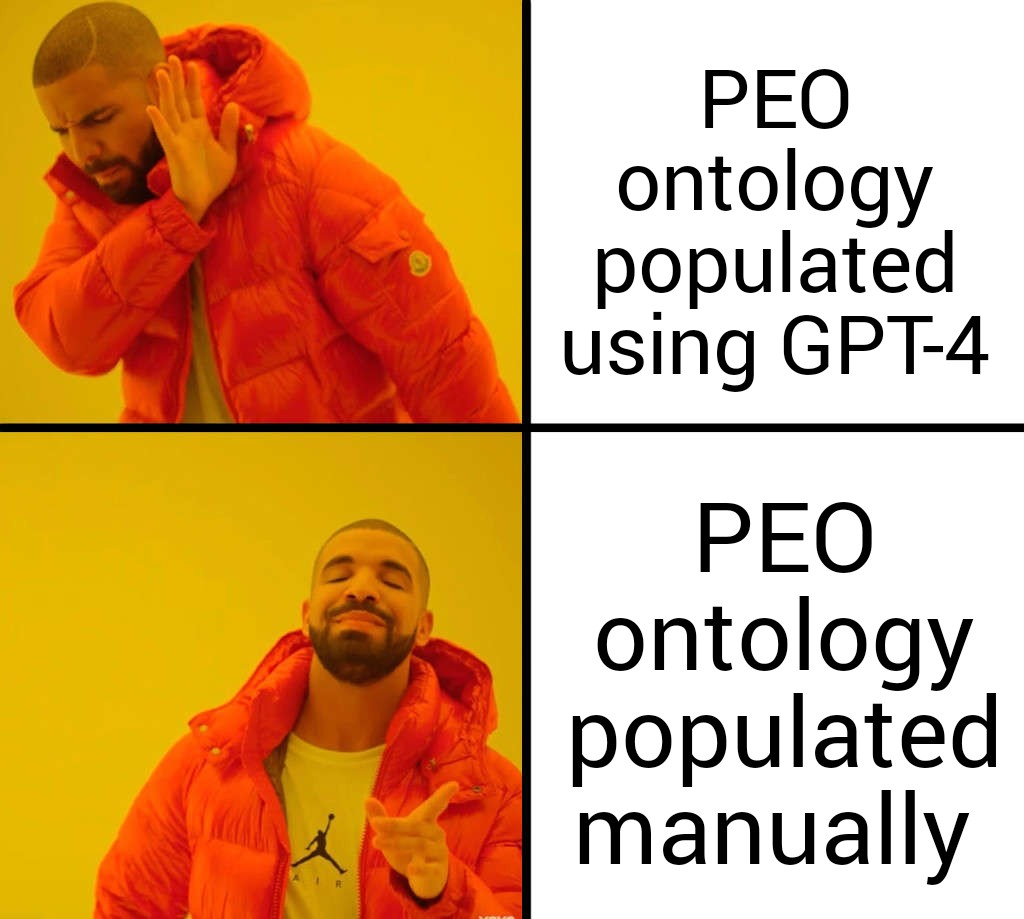
\includegraphics[width=0.36\linewidth]{Figures/fig_64.jpg}
    \caption{Ontology version choosing}
    \label{fig:enter-label}
\end{figure}

\subsection{Ontology documentation}
The ontology documentation is generated using Protegé and the OWLdoc plug-in which automatically generate HTML documentation starting from ontology code. The output of OWLdoc is the following:
\begin{figure}[H]
    \centering
    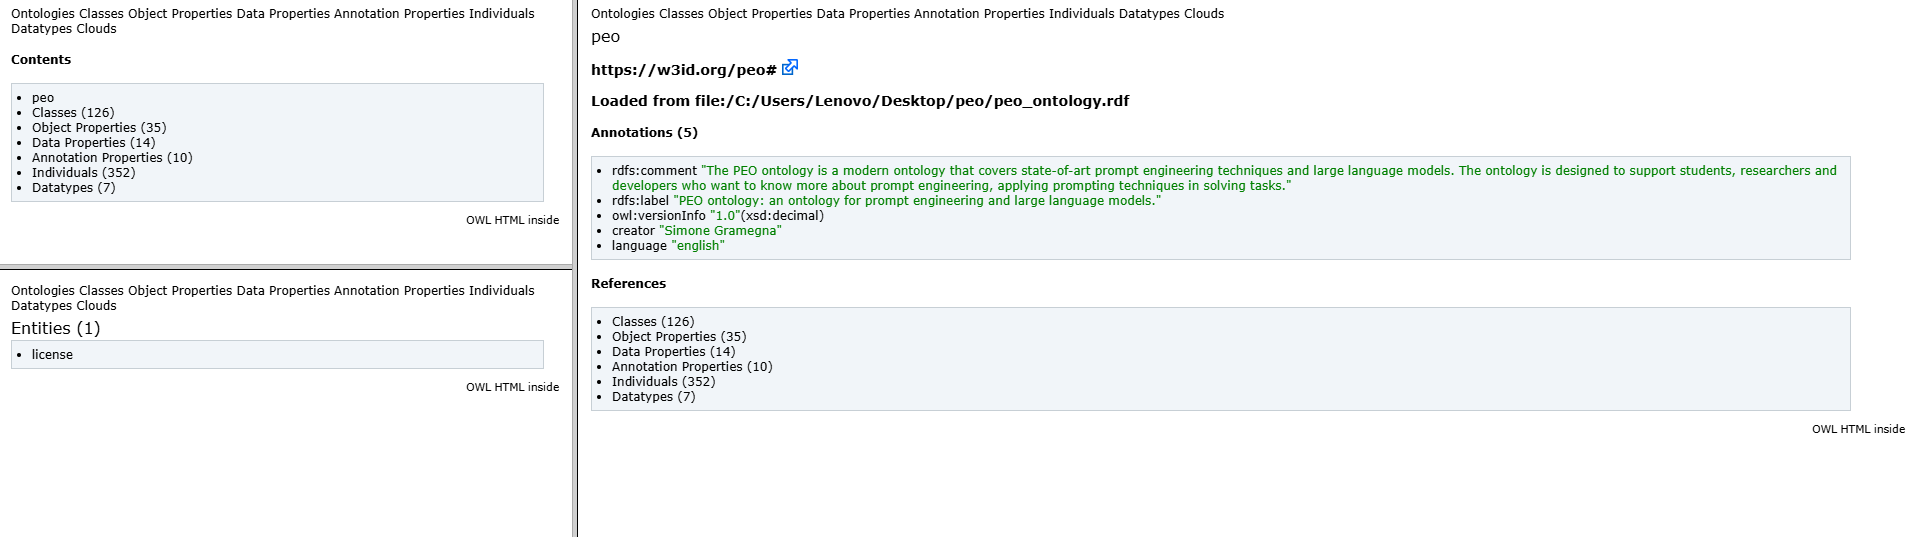
\includegraphics[width=0.9\linewidth]{Figures/fig_63.png}
    \caption{OWLdoc output}
    \label{fig:enter-label}
\end{figure}
The OWLdoc is available in the Github repository \href{https://github.com/simonegramegna/peo/tree/main/docs}{here} in the \textit{/docs} folder and it can be consulted online \href{https://peoontology.vercel.app/}{here}. The documentation is made accessible for everyone using Vercel: a cloud platform for hosting web applications and static sites. This free service using an integrated Github action, takes as input the documentation in the repository and publishes online automatically without requiring any effort by the developer. The \textit{official documentation website} is:
\href{https://peoontology.vercel.app/}{https://peoontology.vercel.app/}.

\subsection{Online publication}
Once the ontology documentation is ready, the ontology can be published online on major vocabularies repository, by accessing the ontology using its URI. I will consider two most known repositories for ontology publishing: \href{https://w3id.org/}{w3id.org} and \href{https://bioportal.bioontology.org/}{BioPortal}.

\subsubsection{W3id.org}
W3id.org a permanent identifier service that provides stable, persistent, and HTTP-resolvable URIs for web resource. The creation of a new identifier for publishing a new ontology is made using Github and the official W3id.org Github repository. The procedure followed is straightforward, first I fork the W3id.org Github repository on my Github, creating a "copy" of the repository. 
\begin{figure}[H]
    \centering
    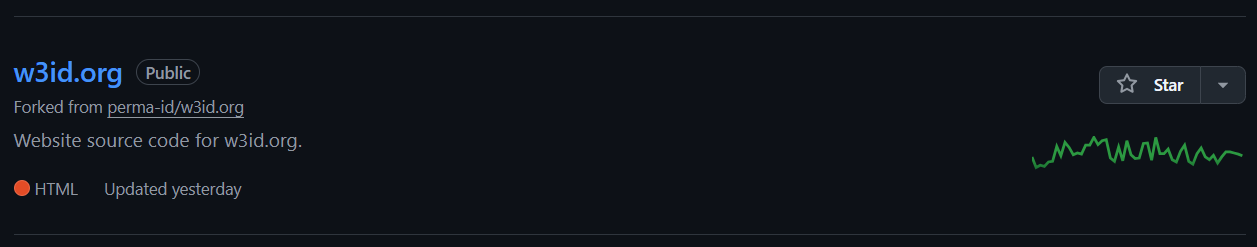
\includegraphics[width=0.9\linewidth]{Figures/fig_65.png}
    \caption{Forked W3id.org repository}
    \label{fig:enter-label}
\end{figure}
Then I create a new branch and I create a new directory with the intended permanent identifier name, in my case I create a directory called \textit{"peo"}. Inside this directory I create two files:
\begin{itemize}
    \item \textit{README.md:} contains more identifier info and contact info, for human to read.
    \item \textit{.htaccess:} contains redirection rules, for computer to read and perform.
\end{itemize}
In the case of PEO ontology, the \textit{README.md} contains all my contact information with the link to the peo Github repository while the \textit{.htaccess} contains the following redirections rules:
\begin{lstlisting}
# Activates Rewrite Engine
RewriteEngine On

# Content negotiation for RDF/XML
RewriteCond %{HTTP_ACCEPT} application/rdf\+xml
RewriteRule ^$ https://raw.githubusercontent.com/simonegramegna/peo/refs/heads/main/peo_ontology.rdf [R=303,L]

# Content negotiation for Turtle
RewriteCond %{HTTP_ACCEPT} text/turtle
RewriteRule ^$ https://raw.githubusercontent.com/simonegramegna/peo/refs/heads/main/peo_ontology.ttl [R=303,L]

# Default: serves HTML for browser or client not RDF-aware
RewriteRule ^$ https://peoontology.vercel.app/ [R=303,L]

# Blocks directory indexing
Options -Indexes
\end{lstlisting}
Once the two files are completed, I submitted a pull request to the main branch that is approved by one of repository administrators. As soon the merge of the created branch, it is possible to access to the ontology using its URI, in the case of PEO ontology the URI is: \href{https://w3id.org/peo}{https://w3id.org/peo} bringing the user with an HTTP request to the online ontology documentation.
\begin{figure}[H]
    \centering
    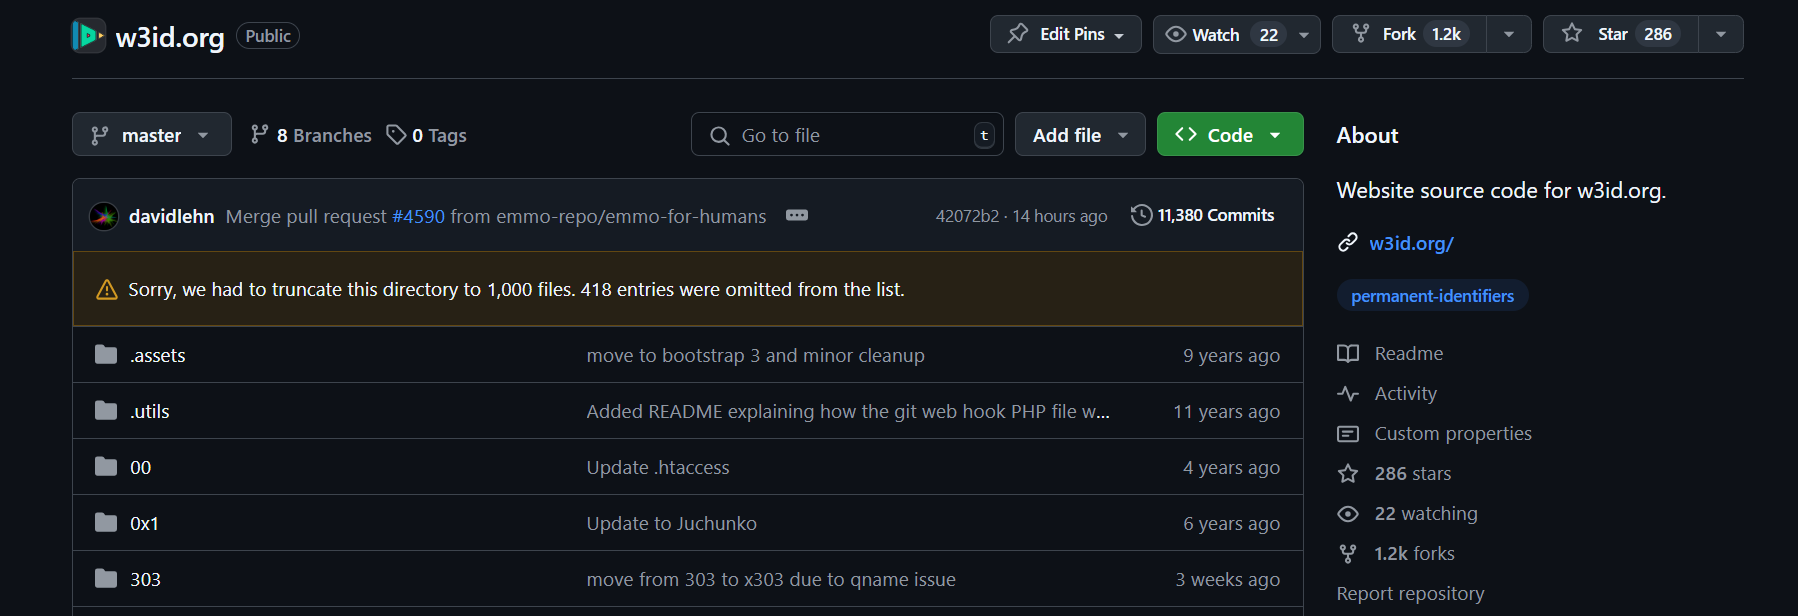
\includegraphics[width=0.9\linewidth]{Figures/fig_66.png}
    \caption{W3id.org repository main directory}
    \label{fig:enter-label}
\end{figure}

\subsubsection{BioPortal}
BioPortal is a  web-based platform designed for the management, exploration, and publication of biomedical ontologies, during the years it has become popular among ontology engineers choosing it as a repository for the publication of different types of ontologies not only in biomedical field. BioPortal offers developers a simple and intuitive interface to publish an ontology, providing the ability to track various versions and visits to the ontology. First I created an account on BioPortal and then I specified all the informations about the ontology: the version, the type (RDF) and the release date. I also specified my contact informations like the e-mail and the Github repository.
\begin{figure}[H]
    \centering
    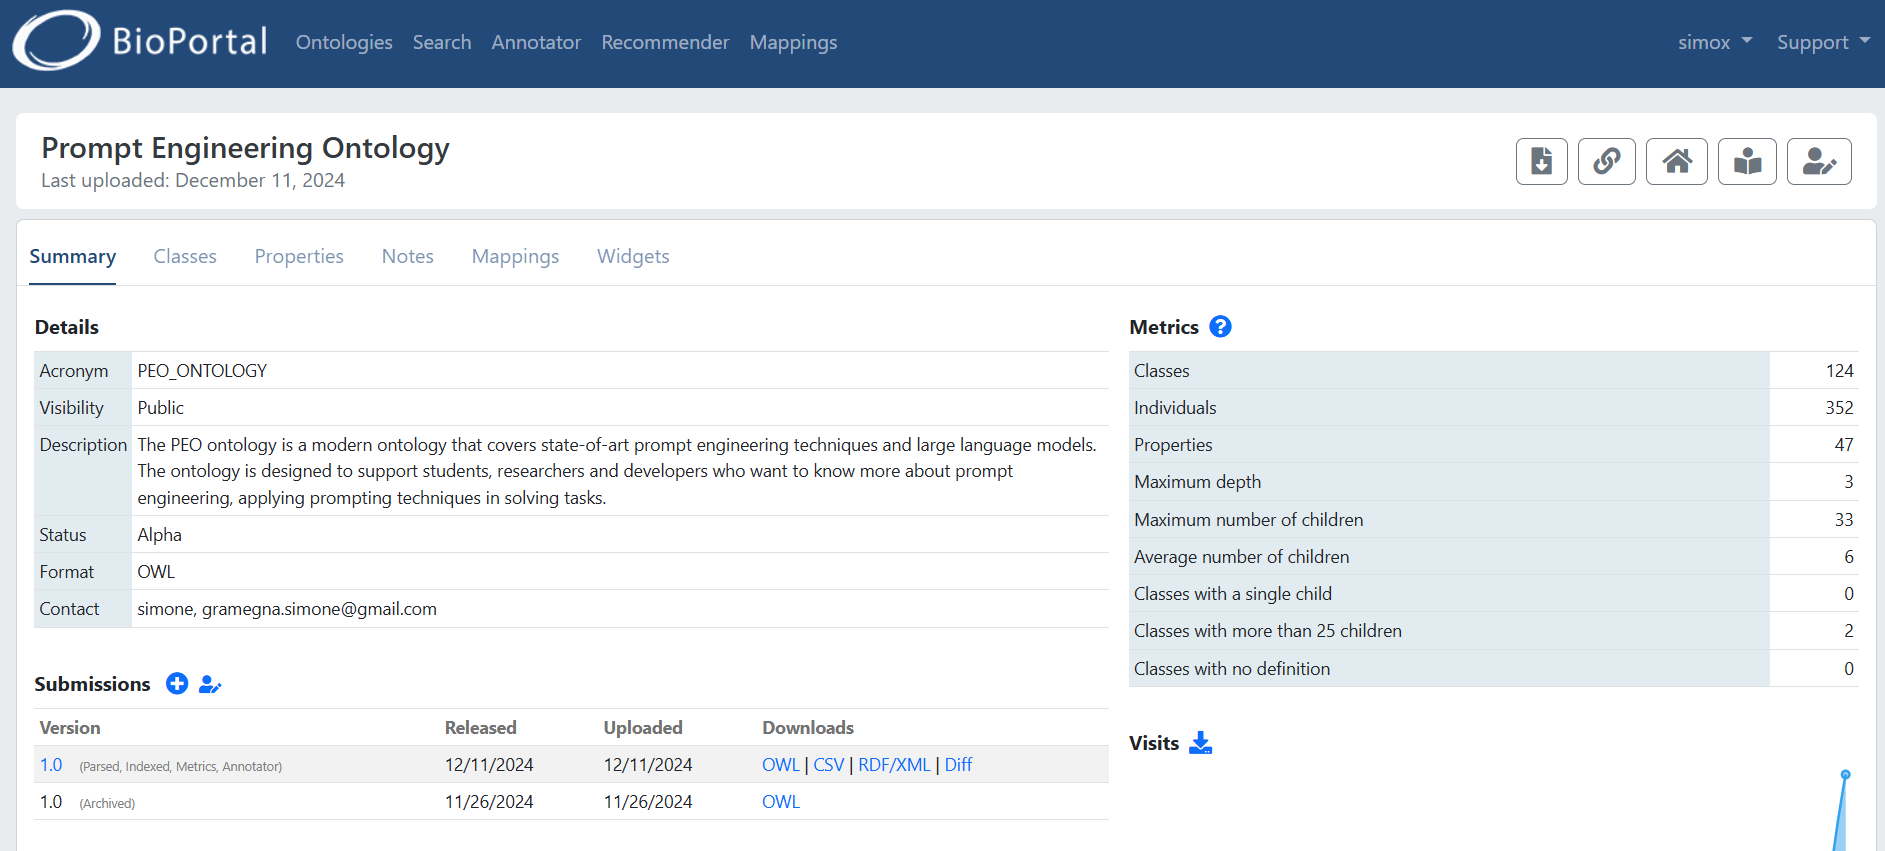
\includegraphics[width=0.9\linewidth]{Figures/fig_67.png}
    \caption{BioPortal main page}
    \label{fig:enter-label}
\end{figure}
The ontology is published at the link \href{https://bioportal.bioontology.org/ontologies/PEO_ONTOLOGY?p=summary}{here} and it is possible using the web interface view the whole ontology: classes, object properties, data properties and individuals. This is a very useful feature because the user has no need to download any additional software, moreover BioPortal computes automatically base ontology metrics. 
\begin{figure}[H]
    \centering
    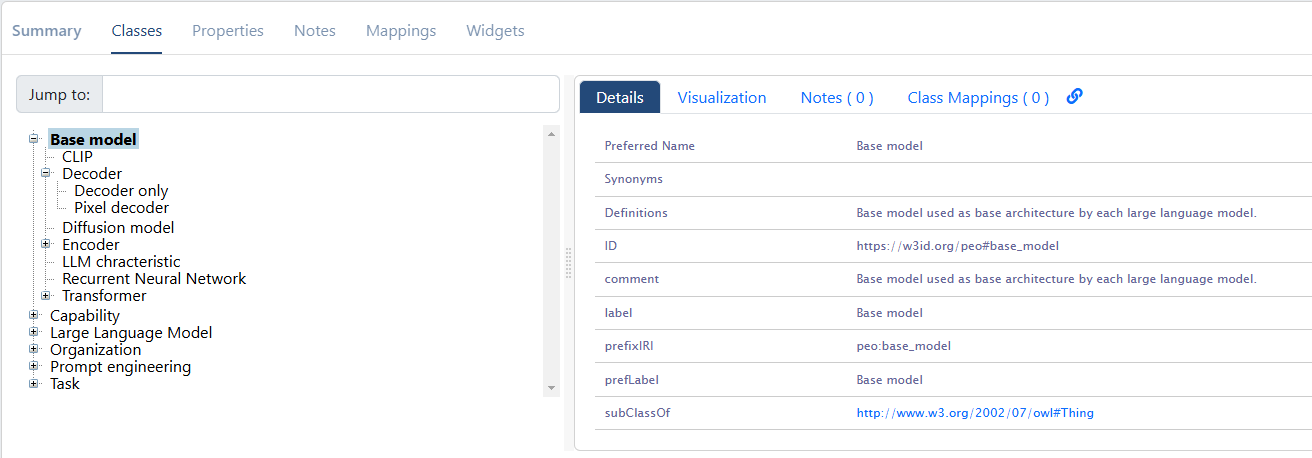
\includegraphics[width=0.9\linewidth]{Figures/fig_68.png}
    \caption{BioPortal ontology interface}
    \label{fig:enter-label}
\end{figure}


\newpage
\section{Ontology maintenance}
The ontology maintenance is the phase that concludes the iteration of the ontology development process, the goal of this phase is to update the ontology during its life cycle. This phase in the case of prompt engineering ontology is important, prompting techniques and large language models are constantly evolving, and regularly updating the ontology is essential to keep it aligned with the latest technologies introduced.\\
In cases where the necessary changes significantly alter the structure of the ontology, it is advisable to formulate new functional requirements through updated competency questions that align with the changes to be introduced. Changes may lead not only to updates but also to the introduction of bugs and pitfalls, which can be identified through the evaluation techniques previously discussed and resolving these issues ensures the quality of the ontology. In general, monitoring and maintaining the traceability of the requirements, bugs and suggestions identified in this activity allows storing discussions and decisions taken that can be later reused. The LOT methodology is designed to support those practices aligned with modern software engineering methodology like the agile methodology from whose iterativity it draws inspiration.

\begin{figure}[H]
    \centering
    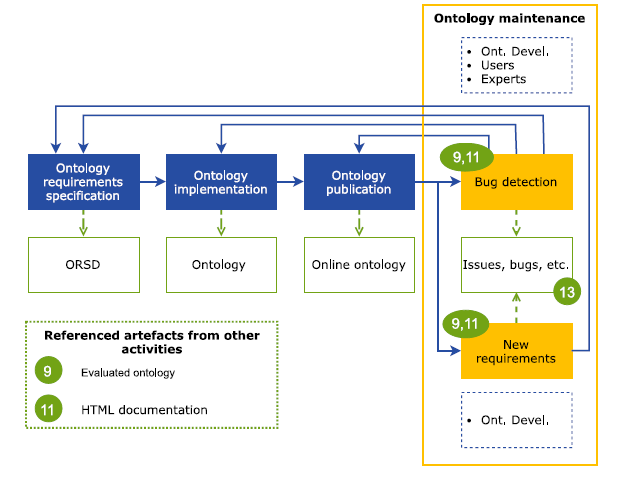
\includegraphics[width=0.9\linewidth]{Figures/fig_33.png}
    \caption{Ontology maintenance workflow}
    \label{fig:enter-label}
\end{figure}

\newpage
\section{Results discussion}






